\documentclass[12pt,a4paper]{article} % 12pt font, A4 paper
\usepackage{graphicx} % Required for inserting images
\usepackage{hyperref}
% Packages for margins and spacing
\usepackage[margin=25mm]{geometry}   % Set all margins to 25 mm
\usepackage{setspace}                % For line spacing control
\usepackage{mathptmx}                % Optional: Use Times as a legible font (can omit for default Computer Modern)
\usepackage{amssymb}
\usepackage{amsmath}
\usepackage{tikz}
\usepackage{pdfpages}

\newcommand{\ve}[1]{\underset{\sim}{#1}}

\setlength{\parskip}{1em}
\setlength{\parindent}{0pt}

% Set 1.5 line spacing
\onehalfspacing

\makeatletter
\renewcommand{\refname}{}
\makeatother

\begin{document}

% \includepdf[pages=-]{cover.pdf}

\begin{titlepage}
    \centering
    \includegraphics[width=.7\linewidth]{unsw.png}
    \vspace{1cm}

    {\LARGE\bfseries Graph Signal Processing}
    \vspace{0.5cm}

    {\large Zac Petersen} \\
    \vspace{0.5cm}
    {School of Electrical Engineering and Telecommunications} \\
    \vspace{0.5cm}
    {Submitted \today}

\end{titlepage}

\pagenumbering{gobble}
\begin{center}
    \subsection*{Abstract}
\end{center}
Graph signal processing is a dense field of research that covers a wide array of problems. Much of its development is built upon the application of traditional signal processing techniques to the graphical domain, but much development is unique entirely to graphical data. Many such techniques have been developed across disciplines; statistics, geography, computer science, discrete mathematics, and signal processing. They apply to a number of problems; compression, prediction, filtering, and computer vision. This report is a preliminary review of a variety of work in these fields and problems over the past century. It works to critique, expand on, link, and reproduce the results of a variety of these works. More broadly, this thesis will aim to produce tangible evidence of the applicability of graph signal processing to a variety of real-world problems, as well as provide novel explanations for their applicability. It will further develop generic techniques for solving problems using graph signal processing problems.

\newpage
\pagenumbering{arabic}
\setcounter{page}{1}
\section*{Acknowledgements}
I would like to thank my supervisor, Professor V. Solo, for pushing me in the right direction, exposing me to appropriate literature, and offering insights orthogonal to my own.

\newpage
\section*{Abbreviations}
\begin{tabular}{cc}
    \textbf{FFT} & Fast Fourier Transform \\
    \textbf{DFT} & Discrete Fourier Transform \\
    \textbf{GFT} & Graph Fourier Transform \\
    \textbf{MSE} & Mean Squared Error \\
    \textbf{RMSE} & Root Mean Squared Error \\
    \textbf{WSS} & Wide Sense Stationary \\
    \textbf{PCA} & Principle Component Analysis \\
    \textbf{SNR} & Signal to Noise Ratio \\
    \textbf{SGD} & Stochastic Gradient Descent \\
    \textbf{BIC} & Bayesian Information Criterion \\
    \textbf{AR}  & Autoregression \\
    \textbf{VAR} & Vector Autoregression
\end{tabular}
\newpage
\tableofcontents

\newpage
\section{Introduction}
Graphs were first introduced into the literature through Euler's solution to the K\"{o}nigsberg bridge problem in 1741 \cite{euler}. Through the ages, graph theory became relevant to a variety of problems including circuit theory, chemistry, and eventually computer science. Many of these original problems are naturally represented by graphs, but many problems on continuous spaces are simplified by endowing them with a graph structure. One of the earliest such examples is the statistical technique invented by Krige to estimate mineral deposit concentration based on a limited number of samples from boreholes \cite{krige}. Despite the age of this field, techniques are not well known, sometimes reinvented across different fields in different forms, and have not uniformly been assessed in practical circumstances.

The present literature has established techniques for compression \cite{moura}, prediction \cite{krige}, filtering \cite{taubin}, and computer vision \cite{grady_shah} on graphs. Such techniques have been relevant to highly influential areas, including advertising and ranking as in the Google PageRank algorithm \cite{page}, risk and stability analysis in econometrics \cite{acemoglu}, and the application of graph techniques to neural networks as has been used in drug discovery and development \cite{sun}. We will explore examples and replicate some of these techniques.

In this report, we replicate techniques and empirically confirm results both with synthetic data sets and a real data set. Two real datasets are used: homogenised daily mean temperature data across Australia as reported by the Bureau of Meteorology (BOM) \cite{bom}, and daily mean temperature data over north America, extracted as a subset of the global surface temperature data provided by the National Oceanic and Atmospheric Administration of the United States (NOAA) \cite{noaa}. The BOM dataset is broadly used for developing and exhibiting methods covered, whilst the NOAA dataset is used to validate the broad utility of models created, as well as to investigate how model parameters change over different samples of the same type of data (temperature networks).

\newpage
\section{Background}\subsection{An Introduction to Graphs, Graph Signals, and Graph Spectra}
\label{subsec:graph_intro}
A graph is a collection of vertices, $\mathcal{V}$, and edges (pairs of vertices), $\mathcal{E}$\footnote{Graphs are made up of 0-dimensional components (vertexes) and 1-dimensional components (edges). Generalised graphs with up to $n$-dimensional components are introduced as $n$-complexes, and addressed in great depth in Grady, 2010 \cite{grady}.}. In some applications, edges may be ordered pairs (directed graphs), but for the purposes of this introduction we consider unordered pairs (undirected graphs). Graph structure is often encoded in an adjacency matrix. For a graph with $n$ vertices, the adjacency matrix is the $n\times n$ matrix $A$ such that $A_{ij}=w_{ij}$, the weight of the edge connecting vertices $v_i$ and $v_j$, or $0$ if there is no such edge.

A graph signal is an association of either each vertex $v\in\mathcal{V}$, or each edge $e\in\mathcal{E}$ with some value. This value could be a scalar, vector, or some other value. In spatiotemporal applications, as are addressed in the following sections, each vertex is associated with a time series. For this introduction, we consider scalar data associated with each vertex.

Graph spectra have been covered extensively in the literature \cite{moura}\cite{mand}. To justify graph spectra, we first cover one reason why the typical Fourier transform is useful. In the continuous domain, the Fourier transform is a mapping from functions in the trivial "shifted-deltas" basis into an orthonormal eigenbasis of the derivative operator (complex exponentials). Because derivatives occur extensively in nature, this proves to be a useful decomposition. Additionally, because of the FFT, the DFT can be implemented quickly, in $O(n\log n)$ time.

A key difference between a graph domain and a discrete time domain is that time has a direction. The first order derivative in time, $\frac{d}{dt}$ measures output changes for increasing time. Because there is no specified "increasing" direction, this is not helpful on an undirected graph. We may turn to multivariate calculus to search for isotropic (directionless) scalar to scalar differential forms. The most obvious is the Laplacian $\nabla^2$, which in the time domain (equivalent to $\frac{d^2}{dt^2}$) has sines and cosines as its eigenfunctions. The integral form of the Laplacian is given below.
\begin{align*}
    \nabla^2f(\ve{x})&=\lim_{h\to0}\frac{2n}{S_nh^{n+1}}\int_{\partial B_{n,h}}f(\ve{y})-f(\ve{x})d\ve{y}
\end{align*}
For $S_n$ the surface area of a unit $n$-ball, and $B_{n,h}$ an $n$-ball with radius $h$. Up to scaling this is a comparison of the values around a point and the value at the point, measuring curvature. In the context of graphs, we associate each edge with some weighting, $w_{ij}$, and assume that some graph signal approximates a signal in a continuous space, where the weighting measures "similarity" or "closeness" of vertices. When the weight is the reciprocal of distance, the negative Laplacian is approximated by the Laplacian matrix, defined below.
\[
    L_{ij}=\begin{cases}
        \sum_{e_{ik}\in\mathcal{E}}\frac{1}{w_{ik}}&\text{if }i=j\\
        -\frac{1}{w_{ij}}&\text{if }i\neq j
    \end{cases}
\]
Note that in this context graph data may be represented by a vector $\textbf{x}$ of the signal value at vertex $v_i$. We then define the GFT as the transformation that takes a graph signal into an orthonormal basis for the Laplacian. Again notice that when operating on one point (e.g. $v=(1\text{ }0\text{ ... }0)^\top$, this compares the value at some vertex to the values at adjacent vertices, up to scaling. Since in the time domain $\nabla^2\cos(\omega t)=-\omega^2\cos(\omega t)$, and the Laplacian matrix represents the Laplacian operator up to a negative constant, the eigenvalues of the equation $\mathbf{Lx}=\lambda\mathbf{x}$ are said to correspond to a frequency (or spatially, wavenumber) of $\sqrt{\lambda}$. That is, the units of $\lambda$ are the inverse square of the units of the edge weights \cite{mand}. Given the decomposition $L=V\Lambda V^{-1}$, the GFT is equivalent to $V^{-1}$.

The GFT can be derived in another way, again adjacent to traditional signal processing. Instead of being framed in terms of the derivative, as in the continuous case, the DFT can be described as a mapping into the eigenbasis of the shift operator, $z^{-1}$ \cite{moura}. We can represent the discrete time domain in this context as a circular domain, where the shift moves a unit impulse around the loop. The relevant directed graph for the time domain is shown in Fig. \ref{fig:cycle12}. The derivation of the GFT in this context simply requires the definition of a shift operator. Typically, choices of a shift operator will involve spreading an impulse at a vertex between neighbouring vertices, as in Fig. \ref{fig:impulse}.

\begin{figure}[!ht]
    \centering
    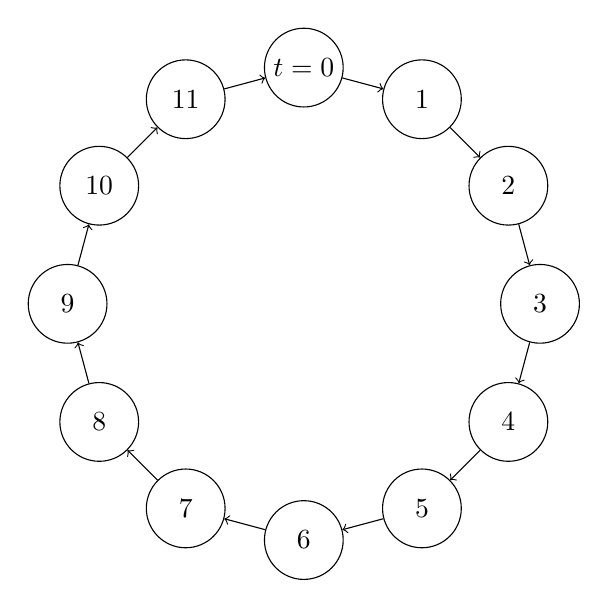
\begin{tikzpicture}
        % Place 12 nodes in a circle
        \foreach \i in {0,...,11} {
            \node[circle, draw, inner sep=2pt, minimum size=10mm] (n\i) at ({-360/12 * (\i-3)}:3) 
                {\ifnum\i=0 $t=0$\else $\i$\fi};
        }
        % Draw directed edges between consecutive nodes
        \foreach \i in {0,...,10} {
            \draw[->] (n\i) -- (n\the\numexpr\i+1\relax);
        }
        % Close the loop from n12 to n1
        \draw[->] (n11) -- (n0);
    \end{tikzpicture}
    \caption{A graph for a time-domain with 12 samples.}
    \label{fig:cycle12}
\end{figure}

\begin{figure}[!ht]
    \centering
    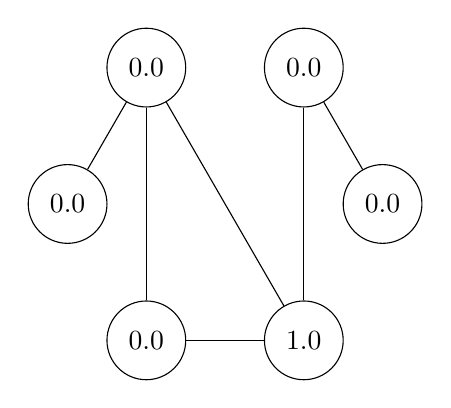
\begin{tikzpicture}[baseline={(0,0)}]
        \node[circle, draw, inner sep=2pt, minimum size=10mm] (n1) at (180:2) {0.0};
        \node[circle, draw, inner sep=2pt, minimum size=10mm] (n2) at (240:2) {0.0};
        \node[circle, draw, inner sep=2pt, minimum size=10mm] (n3) at (300:2) {1.0};
        \node[circle, draw, inner sep=2pt, minimum size=10mm] (n4) at (0:2) {0.0};
        \node[circle, draw, inner sep=2pt, minimum size=10mm] (n5) at (60:2) {0.0};
        \node[circle, draw, inner sep=2pt, minimum size=10mm] (n6) at (120:2) {0.0};
        % Add random undirected edges
        \draw (n1) -- (n6);
        \draw (n6) -- (n2);
        \draw (n6) -- (n3);
        \draw (n2) -- (n3);
        \draw (n3) -- (n5);
        \draw (n4) -- (n5);
    \end{tikzpicture}
    \hspace{0.5cm}
    $\to$
    \hspace{0.5cm}
    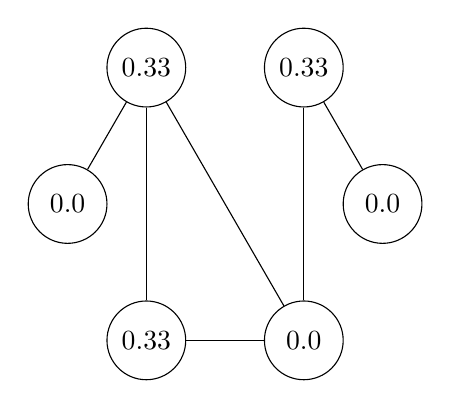
\begin{tikzpicture}[baseline={(0,0)}]
        \node[circle, draw, inner sep=2pt, minimum size=10mm] (n1) at (180:2) {0.0};
        \node[circle, draw, inner sep=2pt, minimum size=10mm] (n2) at (240:2) {0.33};
        \node[circle, draw, inner sep=2pt, minimum size=10mm] (n3) at (300:2) {0.0};
        \node[circle, draw, inner sep=2pt, minimum size=10mm] (n4) at (0:2) {0.0};
        \node[circle, draw, inner sep=2pt, minimum size=10mm] (n5) at (60:2) {0.33};
        \node[circle, draw, inner sep=2pt, minimum size=10mm] (n6) at (120:2) {0.33};
        % Add random undirected edges
        \draw (n1) -- (n6);
        \draw (n6) -- (n2);
        \draw (n6) -- (n3);
        \draw (n2) -- (n3);
        \draw (n3) -- (n5);
        \draw (n4) -- (n5);
    \end{tikzpicture}
    \caption{A impulse spreading to nearby nodes under a particular shift operator.}
    \label{fig:impulse}
\end{figure}

Note that these two methods provide entirely different definitions of the GFT. This is common throughout the literature, and there are yet more ways to define the graph Laplacian.

\newpage
\section{Literature Review}
\subsection{Graph Products and Fast GFTs}
\label{subsec:graph_product}
Part of the ubiquitous utility of the DFT across data science, algorithms, and engineering, is that it may be sped up significantly from na\"{i}ve $O(n^2)$ time to $O(n\log n)$ time by the FFT. Underpinning the FFT is the division of the DFT into the DFT into a number of components. In particular, the speed up relies upon the splitting of the domain into subdomains for each prime factor of the size of the DFT \cite{cooley}. The most common FFT algorithm, the Cooley-Tukey algorithm, offers no speed up for a DFT over a time domain whose length is prime.

We may hope then, that we can speed up the GFT for many graphical domains. Moura, 2014 \cite{moura}, links products of domain sizes for the DFT to graph products of time-domain graphs as was described in \ref{subsec:graph_intro}. Spatiotemporal data is shown to be representable as a graph product, such that not only do values at future time steps depend on the previous time step at the same location, but also at neighbouring locations in the previous time step via the strong graph product, as in Fig. \ref{fig:strong_product}.
\begin{figure}[!ht]
    \centering
    \begin{tikzpicture}[baseline={(0,0)}]
        \node[circle, draw, inner sep=2pt, minimum size=5mm] (n1) at (0,0) {};
        \node[circle, draw, inner sep=2pt, minimum size=5mm] (n2) at (0,2) {};
        \node[circle, draw, inner sep=2pt, minimum size=5mm] (n3) at (1,-1.73) {};
        \node[circle, draw, inner sep=2pt, minimum size=5mm] (n4) at (-1,-1.73) {};
        \draw (n1) -- (n2);
        \draw (n1) -- (n3);
        \draw (n1) -- (n4);
    \end{tikzpicture}
    \hspace{0.5cm}
    $\boxtimes$
    \hspace{0.5cm}
    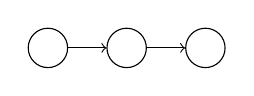
\begin{tikzpicture}[baseline={(0,0)}]
        \node[circle, draw, inner sep=2pt, minimum size=5mm] (n1) at (0,0) {};
        \node[circle, draw, inner sep=2pt, minimum size=5mm] (n2) at (1,0) {};
        \node[circle, draw, inner sep=2pt, minimum size=5mm] (n3) at (2,0) {};
        \draw[->] (n1) -- (n2);
        \draw[->] (n2) -- (n3);
    \end{tikzpicture}
    \hspace{0.5cm}
    $=$
    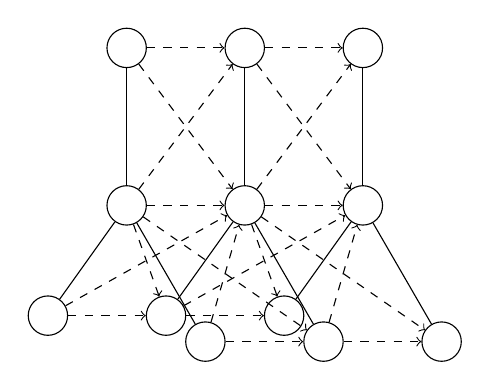
\begin{tikzpicture}[baseline={(0,0)}]
        \node[circle, draw, inner sep=2pt, minimum size=5mm] (n1) at (0,0) {};
        \node[circle, draw, inner sep=2pt, minimum size=5mm] (n2) at (0,2) {};
        \node[circle, draw, inner sep=2pt, minimum size=5mm] (n3) at (1,-1.73) {};
        \node[circle, draw, inner sep=2pt, minimum size=5mm] (n4) at (-1,-1.4) {};
        \node[circle, draw, inner sep=2pt, minimum size=5mm] (n5) at (1.5,0) {};
        \node[circle, draw, inner sep=2pt, minimum size=5mm] (n6) at (1.5,2) {};
        \node[circle, draw, inner sep=2pt, minimum size=5mm] (n7) at (2.5,-1.73) {};
        \node[circle, draw, inner sep=2pt, minimum size=5mm] (n8) at (0.5,-1.4) {};
        \node[circle, draw, inner sep=2pt, minimum size=5mm] (n9) at (3,0) {};
        \node[circle, draw, inner sep=2pt, minimum size=5mm] (n10) at (3,2) {};
        \node[circle, draw, inner sep=2pt, minimum size=5mm] (n11) at (4,-1.73) {};
        \node[circle, draw, inner sep=2pt, minimum size=5mm] (n12) at (2,-1.4) {};
        \draw (n1) -- (n2);
        \draw (n1) -- (n3);
        \draw (n1) -- (n4);
        \draw (n5) -- (n6);
        \draw (n5) -- (n7);
        \draw (n5) -- (n8);
        \draw (n9) -- (n10);
        \draw (n9) -- (n11);
        \draw (n9) -- (n12);

        \draw[dashed, ->] (n1) -- (n5);
        \draw[dashed, ->] (n5) -- (n9);

        \draw[dashed, ->] (n2) -- (n6);
        \draw[dashed, ->] (n6) -- (n10);

        \draw[dashed, ->] (n3) -- (n7);
        \draw[dashed, ->] (n7) -- (n11);

        \draw[dashed, ->] (n4) -- (n8);
        \draw[dashed, ->] (n8) -- (n12);
        %%
        \draw[dashed, ->] (n4) -- (n5);
        \draw[dashed, ->] (n1) -- (n8);

        \draw[dashed, ->] (n8) -- (n9);
        \draw[dashed, ->] (n5) -- (n12);

        \draw[dashed, ->] (n3) -- (n5);
        \draw[dashed, ->] (n1) -- (n7);

        \draw[dashed, ->] (n5) -- (n11);
        \draw[dashed, ->] (n7) -- (n9);

        \draw[dashed, ->] (n1) -- (n6);
        \draw[dashed, ->] (n2) -- (n5);

        \draw[dashed, ->] (n5) -- (n10);
        \draw[dashed, ->] (n6) -- (n9);
    \end{tikzpicture}
    \caption{The strong product of two graphs.}
    \label{fig:strong_product}
\end{figure}
They also show that across three choices of graph product, the overall GFT is the same, only the eigenvalues change. For the two factor graphs with GFTs $A$ and $B$, the product graph has GFT $C$ as below, where $\otimes$ is the Kronecker product of matrices.
\begin{align*}
    C&=A\otimes B
\end{align*}
Note that for moderately sized graphs, this Kronecker product results in an exorbitantly large space complexity. For graph factors with $a$ and $b$ vertices respectively, the GFT matrix $C$ is $a^2b^2$. So this factorisation helps enormously, reducing the space requirement to $a^2+b^2$. Finding the GFT of a graph with $n$ vertices na\"{i}vely requires $O(n^3)$ operations to perform an eigendecomposition of a shift matrix. Moura's method reduces the time complexity in this case from $O(a^3b^3)$ to $O(a^3+b^3)$, a massive saving. Moura does not describe how to perform this GFT quickly, without the need to use the massive $C$ matrix, which gives $O(a^2b^2)$ time. This limitation is addressed in \ref{subsec:efficient_GFT} In fact, the GFT can also be performed faster with this method. The computation time $T_C$ can be reduced to $bT_A+aT_B$. If no more factorisation is available, this gives a complexity of $O(ba^2+ab^2)$, a speed up of $O(a+b)$. Moura notes this speed up for filtering operations, but not for the GFT itself. The matrix-vector product can be represented as below \cite{loan}.
\[
    (A\otimes B) \mathbf{x}=BXA^\top
\]
Where the matrix $X$ represents horizontally stacking $a$ chunks of $\mathbf{x}$ each of size $b$. The left matrix-matrix product is $O(b^2a)$, and the right $O(a^2b)$. This yields an intuitive method for computing the GFT. Since the graph product makes a copy of the graph $B$ for every vertex of $A$, we first run $B$'s GFT on each copy of $B$, and then each eigenvector of $B$'s spectra has a component for every vertex of graph $A$. For each eigenvector, we run $A$'s GFT. In the spatiotemporal case, where we take the graph product of a time domain and a spacial domain, this involves taking the FFT of every vertices' time series, and then taking the GFT for each frequency. For time series of length $a$, and graph with $b$ vertices, this speeds the process up beyond the once-factorable speed to $O(ab^2+ba\log a)$. For small graphs and long time series this is a fairly efficient algorithm.

An important question then is how often are graphs factorable? Some key graphs are factorable. Spatiotemporal data, as we saw, lattices, as in image processing, and toroids, as in the higher-dimensional DFT, are all factorable. It has been shown that, under the Cartesian graph product, factorable graphs can be factorized in linear time \cite{imrich}. A distribution of random graphs can be expressed as a distribution of adjacency matrices. Taking the eigenvectors of these matrices adds an additional degree of randomness. Supposing each entry of each matrix can take on one of $F$ values, given the space complexity requirements, we can propose a crude approximation for the probability of kronecker matrix factorability.
\begin{align*}
    P(\exists A,B:C=A\otimes B)\approx\frac{F^{a^2+b^2}}{F^{a^2b^2}}
\end{align*}
We expect there is a vanishingly small probability of finding a factor in the case of random graphs. Approximate solutions to the equation, that is the nearest-kronecker-product problem have been discussed as a method for dimensionality reduction \cite{loan}, which could prove a useful tool for approximating the GFT in large graphical contexts.

\subsubsection{Application to Compression Problems}
\label{subsec:compression}
Data compression is a fairly universal problem, as data storage is expensive. One method for lossy data compression using the DFT in traditional signal processing involves taking the DFT of a signal, and discarding low-magnitude components. Because eigenvectors describe global structure of the domain, often most of the signal is contained within relatively few eigenvectors. JPEG compression, which is a commonly used image compression technique performs a similar process, using the discrete cosine transform (DCT) rather than the DFT \cite{JPEG}.

Moura applies the fast GFT to compress spatiotemporal daily temperature data across the United States for 150 stations across 1 year (365 measurements) \cite{moura}. A subset of the coefficients of the spatiotemporal GFT eigenvectors are used, selecting the coefficients with largest magnitude. Their results are shown in Fig. \ref{fig:moura-results}.

\begin{figure}[!ht]
    \centering
        \begin{tabular}{|c|c|c|c|c|c|c|c|}
         \hline
         Fraction of Coefficients Used & 1/50 & 1/20 & 1/15 & 1/10 & 1/7 & 1/5 & 1/3 \\
         \hline
         RMSE (\%) & 4.9 & 3.5 & 3.1 & 2.6 & 2.1 & 1.6 & 0.7 \\
         \hline
    \end{tabular}
    \caption{US Data Daily Temperature (2002) Compression Results}
    \label{fig:moura-results}
\end{figure}
Moura does not discuss how much of this compression can be attributed simply to time-domain compression, and how much is due to graph-domain compression. Methods for evaluating this are discussed in the preliminary work in \ref{subsec:efficient_GFT}.

Storing sparse coefficients like this however requires knowledge of the eigenvectors corresponding to each coefficient, as they are not so structures as the eigenvectors of the DFT. This requires storage costs of $n^2$ floats for $n$ weather stations, which in Moura's case represents $150^2/(150\cdot365)\approx41\%$ of the original storage cost. Alternatively, the decompression process can involve finding the GFT matrix through storing the associated graph metadata. I.e. the edges, their weights (or how these were found from for example, location data). The paper assigns edges via a nearest-neighbour scheme, and weights through equation (29) in their preceding paper \cite{moura2}, modified for clarity below. Note $d$ denotes the distances between measurement points, and $\sigma$ denotes a scaling factor.
\begin{align*}
    w_{ij}&=\frac{e^{-d_{ij}^2/\sigma^2}}{\sqrt{\sum_{k:e_{ik}\in\mathcal{E}}e^{-d_{ik}^2/\sigma^2}\sum_{k:e_{jk}\in\mathcal{E}}e^{-d_{jk}^2/\sigma^2}}}
\end{align*}
The choice of nearest-neighbour scheme and the use of a Gaussian kernel rather than some other is unjustified, except to say they their use is common and has shown some success. We will justify other kernels later when discussing the Mat\'{e}rn kernel in \ref{subsec:matern}, and will point out the success of the Gaussian in \ref{subsec:GFT_comparison}.

\subsection{Graph Windowing and Convolution with the GFT}
\label{subsec:graph_convolve}
In time-domain convolution first arises in filter application. A linear time-invariant filter can always be expressed as a convolution of a time signal $x[n]$ with an impulse response $h[n]$ as below.
\begin{align*}
    y[n]&=\sum_{k=-\infty}^\infty x[k]h[n-k]
\end{align*}
Of course, in the graph domain, $n$ and $k$ are vertices, and there is no natural subtraction of vertices. One intuitive option is to call $n-k$ the shortest distance between the vertices. The shortest distance between two vertices in a graph may be found via Dijkstra's algorithm \cite{dijkstra} in $O((V+E)\log E)$, or all distances may be found via the Floyd-Warshall algorithm \cite{floyd} in $O(V^3)$ (for $V$ the number of vertices and $E$ the number of edges). Another prominent method, highlighted by Stankovic et. al. \cite{stankovic}, amongst others, is to note one of the most important properties of time-domain convolution, frequency domain multiplication. In the frequency domain, convolution becomes an elementwise multiplication. So, we can define convolution as follows.
\begin{enumerate}
    \item Take the GFT of $x[n]$ and $h[n]$ to get $X[k]$ and $H[k]$.
    \item Multiply to get $\hat{X}[k]=X[k]H[k]$.
    \item Apply the IGFT to get $\hat{x}[n]=x[n]*h[n]$, the convolution.
\end{enumerate}
Naturally, this requires eigendecomposing a graph operator to get the GFT and IGFT, which as discussed in \ref{subsec:graph_product} can be slow when a graph has many vertices.

As discussed in \ref{subsec:graph_intro}, a graph shift operator is an analog for the time shift operator. That is, just as an impulse response can be represented in terms of its $Z$-transform, which via the convolution formula allows for filter application, some graph filters $\pmb{H}$ can be represented in terms of the graph shift operator $\pmb{A}$, as below.
\begin{align*}
    \pmb{H}&=\sum_{n=-\infty}^\infty h_n\pmb{A}^n
\end{align*}
In particular, a linear graph shift operator most generally is any matrix that applies to the graph signal vector. The graph filters that can be represented in terms of the graph shift operator are in some sense "space invariant", as a time-domain filter may be "time invariant".

In traditional signal processing, more complex data analysis is performed through the use of the short-time Fourier transform, which allows for analysis of frequency data over time. Because the natural domain of the DFT is a toroidal space, that is the beginning is in some sense "attached" to the end, due to the aliasing process of digital sampling, spectral leakage occurs, so windowing is used to provide a more useful estimate of frequency data. Windowing involves elementwise multiplying a time domain signal by a window function, say $w[n]$. Another helpful thing about windowing is that we need not process a whole dataset. Although this is less of a problem in the time domain, as the FFT is fast, in the graph domain, a graph with say a million vertices would be near impossible to eigendecompose. As such, windowing graph data to a local area would be immensely helpful. Stankovic et. al. describe a more ideal circumstance, where the GFT is computed and the windows are defined from there, which allows for local-space analysis. Nevertheless, the option for less ideal windowing remains.

Stankovic et. al. also describe the implementation of graph bandpass filters, to target a particular range of the eigenspectrum, via the chebyshev set of filters, modified via the expansion above to use the graph operator. It is important to note that although general dense matrix multiplication is $O(n^3)$, for sparse matrices, as in the graph operators we have described so far, multiplication is much faster for relatively low powers of $\pmb{A}$, as in $\pmb{A}^k$, $k<<n$. In \ref{subsec:well_chosen_GFT} we discuss an good choice of a low-pass filter on a particular graph operator, though efficient implementation is still difficult. We also discuss how a graph operator should be chosen, and link the low-pass graph filter to the minimum MSE optimal noise reduction filter, the Wiener filter. The theory for the Wiener filter in the time domain is discussed in \ref{subsec:wiener}.

\subsection{Temporal Stochastic Processes; Predictive Filters}
\label{subsec:temporal_processes}
When assessing the utility of spatial modelling for the analysis of spatiotemporal data, it must be evaluated against the use of temporal modelling alone. Temporal modelling is ubiquitous, as being able to predict the future is almost universally a lucrative enterprise. Additionally, temporal modelling provides many techniques that can be applied with modification in the spatial domain. For these reasons, we will introduce temporal stochastic processes and predictive filters.

A stochastic process $X$ is a collection of random variables $X_t\forall t\in\mathbb{R}$. We may have a discrete time domain if instead $t\in\mathbb{Z}$. Because time only flows in one direction, $X_t$ can only depend upon random noise, as well as $X_\tau\forall\tau\leq t$.

A stochastic process $X$ is considered stationary if the distribution of $X_t$ is independent of $t$. Such a process is further called wide-sense stationary (WSS) if $\text{Cov}(X_t,X_{t-\tau})$ is independent of $t$ \cite{stochastic_wiki}.

In the discrete domain, linear regression (discussed in \ref{subsec:lse}) can be used to regress a signal against its past values. This gives an optimal (in the MSE sense) linear deterministic predictive filter.

Examples of more sophisticated filters include the Wiener and Kalman filters, both adaptive (non-deterministic) filters \cite{wiener}.

As a note on the appropriate application of linear regressive models, we recall the first-order model for some signal $T$ and noise $\epsilon$.
\begin{align*}
    T_{t}&=\xi_0T_{t-1}+\epsilon_t\\
    &=\xi_0^2T_{t-2}+\xi_0\epsilon_{t-1}+\epsilon_t\\
    &...\\
    &=\xi^N_0T_{t-N}+\sum_{i=0}^{N-1}\xi_0^i\epsilon_{t-i}
\end{align*}
This means that $T$ can be given as a sum of random variables $\epsilon_\tau$ drawn from the same random distribution, along with a scaling factor. When autoregression explains the data well, $\xi_0\approx1$, so the central limit theorem approximately applies, making $T$ more normally distributed. When the $\xi_0=0$, $T$ is drawn from the same distribution as $\epsilon_\tau$. As such, autoregression tends to be more successful on Gaussian data. Higher order filters can address more complex distributions. Another set of important filters are autoregressive moving average (ARMA) filters, but for brevity we will not discuss these.

\subsection{Continuous-Domain Spatial Stochastic Processes}
\label{subsec:continuous_processes}
Temporal stochastic processes discuss random signals $X_t$ dependent on a time $t\in\mathbb{R}$. Spatial stochastic processes discuss random signals $X_{\ve{x}}$ dependent on a position in space $\ve{x}\in\mathbb{R}^n$. Spatial stochastic processes occur throughout nature. Geostatistical processes, like the distribution of trees, hills, and other geographic features are examples of a single realisation of a spatial stochastic process. Just like in the time domain, the ability to predict/interpolate spatial features allows for significant cost savings in sampling.

Just as in the discrete domain we constrict $t$ to $t\in\mathbb{Z}$, space is often discretised either via the lattice $\mathbb{Z}^n$, or by a graph. Just as time is sampled for practical reasons, so too is the continuous spatial domain often sampled. Spatial discretisations often come in the form of graphs. To do analysis effectively on graphs, it will serve us well to understand the analytical results from continuous-domain spatial stochastic processes.
\subsubsection{The Mat\'{e}rn Kernel}
\label{subsec:matern}
Mat\'{e}rn (1960) discusses stationary spatial stochastic processes \cite{matern}. Here, stationarity means the distribution looks identical around any point in space. In particular, Mat\'{e}rn shows that for a natural extension of type-III probability density functions (a popular broad class of probability density functions including Normal distributions and other common distributions) onto spatial processes, the correlation function between points $\ve{x}$ and $\ve{y}$ is given as below.
\begin{align*}
    \rho(\ve{x},\ve{y})&=\text{const. }||\ve{x}-\ve{y}||_2^\nu K_\nu(\lambda||\ve{x}-\ve{y}||_2)
\end{align*}
For parameters $\nu$ and $\lambda$, and $K_\nu$ the modified bessel function of the second kind with order $\nu$. This kernel is isotropic, so that its covariance is radially symmetric, because it only depends on the distance between $\ve{x}$ and $\ve{y}$.

Whittle (1954) finds a case where the Mat\'{e}rn kernel naturally arises \cite{whittle2}. Working from the discrete domain, he arrives at an equation equivalent to the one below.
\begin{align*}
    (\nabla^2-\lambda^2)X_{\ve{x}}&=\varepsilon_{\ve{x}}
\end{align*}
For $\varepsilon_{\ve{x}}$ uncorrelated white noise. We revisit this model in the preliminary work in \ref{subsec:spatial_model}. In two dimensions ($\nabla^2=\frac{\partial^2}{\partial x^2}+\frac{\partial^2}{\partial y^2}$) he found the correlation function to be a Mat\"{e}rn kernel with $\nu=1$, as below.
\begin{align*}
    \rho(\ve{x},\ve{y})&=\lambda||\ve{x}-\ve{y}||_2 K_1(\lambda||\ve{x}-\ve{y}||_2)
\end{align*}
In his later work, he found the correlation function in all dimensions, except $n=1$, which is addressed in the preliminary work in \ref{subsec:1d_correlation} \cite{whittle}. For $r=||\ve{x}-\ve{y}||_2$, the correlation function $\rho$ is as below.
\begin{align*}
    \rho(r)&=\frac{2^{n/2-1}}{\Gamma(2-n/2)}(\lambda r)^{2-n/2}K_{2-n/2}(\lambda r)
\end{align*}
This model breaks down when $n>4$. Intuitively, the diffusion equation in $5$ or more dimensions has in some sense too many dimensions to diffuse through, so that variance at each point goes to infinity, as noise throughout the space increases the signal variance at each point.
\subsubsection{Kriging}
\label{subsec:kriging}
Kriging is a practical process for spatial interpolation, given a covariance function between points in a space, and a number of samples throughout the space of a realisation of the stationary stochastic process. Kriging was invented by the eponymous Krige, originally proposed for estimation of gold content in the Witwatersrand in South Africa for mine site evaluation \cite{krige}. Since then it has been used across many areas of geostatistical estimation, and also across other many other fields, just one of which is hyperparameter estimation for machine learning methods \cite{hyperkrige}.

There are many methods for empirical estimation of a spatial covariance function, but for brevity we will here assume the covariance function is known. The simplest form of Kriging is simple Kriging, and is equivalent to linearly regressing the data at the interpolation point against the sample points, as discussed in \ref{subsec:linear_reg}. In particular, we consider the spatial process $X_{\ve{x}}$, sampled at $k$ points $\ve{x_i}$, to be interpolated at a point $\ve{y}$. If the sample points have covariance matrix between each other $\pmb{\Sigma}$, and the covariances between the $\ve{x_i}$ and the interpolation point $\ve{y}$ are given in the vector $\ve{\Gamma}:\Gamma_i=\text{Cov}(X_{\ve{x}},X_{\ve{y}})$, then the interpolation $\hat{X_{\ve{y}}}$ is given as below.
\begin{align*}
    \hat{X_{\ve{y}}}&=X_{\ve{x}}^\top\pmb{\Sigma}^{-1}\ve{\Gamma}
\end{align*}
For the vector of samples $X_{\ve{x}}$.
Because the spatial process is stationary, if its mean is $\mu$, we can check the bias of the prediction below.
\begin{align*}
    E(\hat{X_{\ve{y}}})&=E(X_{\ve{x}}^\top)\pmb{\Sigma}^{-1}\ve{\Gamma}\\
    &=\mu\sum_{i=0}^k(\pmb{\Sigma}^{-1}\ve{\Gamma})_i
\end{align*}
So that the process is biased. Finding the least-squares unbiased estimator leads to the ordinary Kriging estimate. The formula below presents the solution, with $\mu$ a Lagrange multiplier that can be discarded.
\begin{align*}
    \begin{pmatrix}
        \hat{\ve{w}}\\
        \mu
    \end{pmatrix}&=\begin{pmatrix}
        \pmb{\Sigma} & \mathbf{1}\\
        \mathbf{1}^\top & 0
    \end{pmatrix}^{-1}\begin{pmatrix}
        \ve{\Gamma}\\
        1
    \end{pmatrix}\\
    \hat{X_{\ve{y}}}&=X_{\ve{x}}^\top \hat{\ve{w}}
\end{align*}
This is the estimate implemented in the preliminary work in \ref{subsec:kriging_implementation}.

The Kriging error is the expected RMSE of the interpolation at each point. In the Ordinary Kriging case it can be computed using the formula below.
\begin{align*}
    \text{Var}(\hat{X_0}-X_0)&=\begin{pmatrix}
        \hat{\ve{w}}^\top&-1
    \end{pmatrix}\begin{pmatrix}
        \pmb{\Sigma} & \ve{\Gamma}\\
        \ve{\Gamma}^\top & \text{Var}(X_0)
    \end{pmatrix}\begin{pmatrix}
        \hat{\ve{w}}\\
        -1
    \end{pmatrix}
\end{align*}

\subsection{Least Squares Estimation}
\label{subsec:lse}
\subsubsection{Linear Regression}
\label{subsec:linear_reg}
Linear regression is one of the simplest and most powerful data fitting techniques. It is often credited to Adrien-Marie Legendre and Carl Friedrich Gauss in their work on predicting planetary movements \cite{linear}. It is common due to its low complexity in terms of the amount of data being processed, being $O(n)$ for $n$ datapoints per feature, and ease of interpretibility due to the simplicity of linear modelling. We cover standard results seen in most statistics textbooks, like \cite{stats}

Linear regression seeks to model some set of $l$ outputs $\ve{y}\in\mathbb{R}^l$, each observed $n$ times and stored in the matrix $\pmb{Y}\in\mathbb{R}^{n\times l}$. It is modelled in terms of a set of $k$ features $\ve{x}\in\mathbb{R}^k$, each of which have again been observed $n$ times and stored in the matrix $\pmb{X}\in\mathbb{R}^{n\times k}$. The relationship is modelled linearly as below.
\begin{align*}
    \pmb{Y}&=\pmb{\beta X} + \pmb{\varepsilon}
\end{align*}
For $\pmb{\beta}\in\mathbb{R}^{k\times l}$ a set of "regression coefficients", where $\pmb{\beta}_{ij}$ encodes how much feature $x_i$ linearly impacts output $y_j$, and $\pmb{\varepsilon}\in\mathbb{R}^{n\times l}$ some error. The error is modelled as normal and 0-mean, because, due to the central limit theorem, normality of error is common if the model is an appropriate one. Then, we seek the maximum-likelihood estimator of $\pmb{\beta}$, such that $\pmb{\hat{\beta}}=\arg\min_{\pmb{\beta}}(P(\pmb{\varepsilon}|\pmb{\beta}))$. Due to normality it can be shown this is equivalent to the least-squared error estimation criteria, i.e. $\pmb{\hat{\beta}}=\arg\min_{\pmb{\beta}}(||\pmb{\varepsilon}||_2^2)$. Using basic matrix calculus techniques, the major result can be shown.
\[
    \pmb{\hat{\beta}}=(\pmb{X}^\top\pmb{X})^{-1}\pmb{X}^\top \pmb{Y}
\]
With the appropriate order of operations, this evaluation has time complexity of order $O(nk^2+k^3+nkl+k^2l)=O(k^2(n+k)+kl(n+k))=O(k(k+l)(n+k))$. Since the model is generally only performant when $n>>k$ and $n>>l$, this model is fairly fast ($O(n)$) for few features and outputs.

One significant way to interpret the solution is covariance estimation. For 0-mean data, $\pmb{X}^\top\pmb{X}\approx \pmb{\Sigma}_{\ve{x}}$, the covariance matrix of $\ve{x}$, and $\pmb{X}^\top\pmb{Y}\approx\pmb{\Gamma}_{\ve{x}\ve{y}}$, the cross-covariance matrix of $\ve{x}$ and $\ve{y}$. So as we see more and more data, that is $n\to\infty$ we can represent the true $\pmb{\beta}$ as below.
\[
    \pmb{\beta}=\pmb{\Sigma}_{\ve{x}}^{-1}\pmb{\Gamma}_{\ve{x}\ve{y}}
\]
\subsubsection{The Wiener Filter}
\label{subsec:wiener}
The Wiener filter is a noise-reduction filter that aims to remove noise subject to least-squares estimation of a desired signal. That is, we have the problem below in $\mathbb{R}^n$.
\[
    \ve{y}(t)=\ve{x}(t)+\ve{\varepsilon}(t)
\]
For 0-mean normal noise $\ve{\varepsilon}(t)$. The assumption of noise normality as discussed in \ref{subsec:linear_reg} gives rise to the least-squares minimisation problem via the maximum likelihood estimation of $\ve{x}(t)$ given $\ve{y}(t)$. The solution to this problem $\hat{\ve{x}}(t)$ can be stated simply in terms of known covariance matrices. The below solution is commonly referred to as the minimum mean-square error estimator \cite{mmse}.
\[
    \hat{\ve{x}}(t)=\pmb{\Sigma}_{\ve{x}}(\pmb{\Sigma}_{\ve{x}}+\pmb{\Sigma}_{\ve{\varepsilon}})^{-1}\ve{y}(t)
\]
For the covariances of $\ve{x}(t)$ and $\ve{\varepsilon}(t)$, $\pmb{\Sigma}_{\ve{x}}$ and $\pmb{\Sigma}_{\ve{\varepsilon}}$ respectively. This filter is said to be adaptive, as its structure depends on the data, which is to say its covariance.

\subsection{Regularisation as Graph Selection}
\label{subsec:intro_reg_as_graph_sel}
In many applications we can consider all pairwise relationships between a set of variables. This corresponds, rather simply to the complete graph of pairwise relationships. In reality, we expect many pairwise relationships to be irrelevant or not useful. In this case, we may wish to prune down the complete graph to a much sparser graph to represent only the useful pairwise relationships. In applications where there is an underlying graph present, this can be useful for identifying missing links, and in other applications it can simplify model structure and reduce size. In particular, for a Gaussian random field, strength of pairwise relationships are identified as the elements of the precision matrix, $\pmb{\Sigma}^{-1}$. Friedman, J. et. al. \cite{friedmanglasso} were the first to do this, applying L1 regularisation to the likelihood function of the inverse covariance matrix. We can derive this likelihood as below for k-dimensional vectors.
\begin{align*}
    \mathcal{N}(\ve{\mu},\pmb{\Sigma})&\sim(2\pi)^{-k/2}\det(\pmb{\Sigma})^{-1/2}\exp(-\frac12 (\ve{x}-\ve{\mu})^\top\pmb{\Sigma}^{-1}(\ve{x}-\ve{\mu}))\\
    P(\ve{x_0},\ve{x_1},\dots,{\ve{x_n}})&=\prod_{i=0}^n(2\pi)^{-k/2}\det(\pmb{\Sigma})^{-1/2}\exp(-\frac12 (\ve{x_i}-\ve{\mu})^\top\pmb{\Sigma}^{-1}(\ve{x_i}-\ve{\mu}))\\
    \ln(P(\ve{x_0},\ve{x_1},\dots,{\ve{x_n}}))&=\sum_{i=0}^n -\frac{k}{2}\ln(2\pi)+\frac12\ln\det(\pmb{\Sigma}^{-1})-\frac12(\ve{x_i}-\ve{\mu})^\top\pmb{\Sigma}^{-1}(\ve{x_i}-\ve{\mu}))\\
    &=const.+\frac{n}{2}(\ln\det(\pmb{\Sigma}^{-1})-\frac{1}{n}\sum_{i=0}^n(\ve{x_i}-\ve{\mu})^\top\pmb{\Sigma}^{-1}(\ve{x_i}-\ve{\mu}))\\
    &\text{up to a constant:}\\
    &=\frac{n}{2}(\ln\det(\pmb{\Sigma}^{-1})-\frac{1}{n}\sum_{i=0}^n(\ve{x_i}-\ve{\mu})^\top\pmb{\Sigma}^{-1}(\ve{x_i}-\ve{\mu}))\\
    &=\frac{n}{2}(\ln\det(\pmb{\Sigma}^{-1})-\text{tr}(\pmb{\Sigma}^{-1}\frac{1}{n}\sum_{i=0}^n(\ve{x_i}-\ve{\mu})^\top(\ve{x_i}-\ve{\mu})))\\
    &=\frac{n}{2}(\ln\det(\pmb{\Sigma}^{-1})-\text{tr}(\pmb{\Sigma}^{-1}S))\\
    &\text{for }S\text{ the sample covariance.}
\end{align*}
Regularisers on the log-likelihood are computationally easier to deal with that those in pure likelihood space, and they have the added advantage of often being connected to a particular prior on the parameters. For example, consider the L1 regularised precision matrix likelihood equation below.
\begin{align*}
    \mathcal{L}&=\ln\det(\pmb{\Sigma}^{-1})-\text{tr}(\pmb{\Sigma}^{-1}S)+\lambda\sum_{i,j}|\pmb{\Sigma}^{-1}_{i,j}|
\end{align*}
It is well known \cite{park} that the L1 regulariser places a Laplacian prior on each parameter independently, that is a priori we consider $P(\pmb{\Sigma}^{-1}_{i,j}=\theta)\propto e^{-\lambda|\theta|}$. With an appropriate prior, such as L1 or L0 regularisation, this leads to zeroing out of some parameters at the maximum likelihood estimator. With a sufficiently stringent prior, this essentially leads to graph selection, as a limited number of pairwise relationships are considered valid, pruning the complete graph of relationships down to a sparser, more managable one.

This method quantifies the graphical relationship between scalar random variables for which many samples are available. The methods do not describe how to handle relationships in a graph with time series or vectors at each vertex, where relationships may include delayed or multivariate effects. Examples of such real world time-series networks would be climatic relationships, where it takes time for the climate in one region to effect another region, or a brain network, where neurons influence each other with a synaptic delay.

A notable extension of this system is for graphs where each node is associated with a vector of scalars, rather than a single scalar, where the covariance becomes a rank-3 tensor, rather than a 2d matrix. Z. Yue et. al. \cite{yue} come up with a fast algorithm for approximate solving of the L0 regularised vector inverse covariance tensor approximation. As it is relevant to this work, we will derive and implement a simpler version of this algorithm, namely the fast algorithm in the case of a regular matrix with scalar entries.
\subsubsection{Fast L0 Spare Inverse Covariance}
First, we recall the log-likelihood function for the error precision matrix $\pmb{\Omega}_\varepsilon$ in terms of the sample error covariance $\pmb{S}$ and number of samples $n$.
\begin{align*}
    \mathcal{LL}&=n\log{\det{\pmb{\Omega}}}-n\text{tr}(\pmb{S}\pmb{\Omega})
\end{align*}
Then, we wish to minimise the BIC of the log-likelihood for the number of parameters $k$, as below.
\begin{align*}
    BIC&=-2\mathcal{LL}+\ln(n)k
\end{align*}
This can be expressed as an $l_0$ regression. To simplify things for the algorithm, we presume that the diagonal elements of $\pmb{\Omega}$ are all non-zero. We can then express the function $F(\pmb{\Omega})$ that we wish to minimise as below.
\begin{align*}
    F(\pmb{\Omega})&\propto -\log{\det{\pmb{\Omega}}}+\text{tr}(\pmb{S}\pmb{\Omega})+\frac{\ln{n}}{2n}\sum_{i\neq j}I(\pmb{\Omega}_{ij}\neq0)
\end{align*}
For simplicity, we call $\frac{\ln{n}}{2n}=\lambda$, as in a typical $l_0$ regression. Note that this comes with a number of parameters equal to $\frac12\sum{i\neq j}I(\pmb{\Omega}_{ij}\neq0)$, because the precision matrix is symettric.

One of the key insights of the coordinate descent optimisation algorithm employed here, is to consider optimising row $i$ and column $i$ together, keeping everything else constant. This contrasts with other algorithms that may optimise either rows individually, columns individually, or entries $ij$ in the matrix individually. Because each set of row and column $i$ represents the relationships with variable $i$, we can swap this row and column with the last row and column in the matrix to simplify the expressions for the matrix structure. After optimisation, the rows and columns can be moved back to where they belong. We hence partition the matrix $\pmb{\Omega}$ to be optimised and the sample covariance $\pmb{S}$ as below.
\begin{align*}
    \pmb{\Omega}&=\begin{pmatrix}
        \pmb{\Omega}_{-i}&\ve{\Omega_{-i,i}}\\
        \ve{\Omega_{-i,i}}^\top&\omega_{i,i}
    \end{pmatrix}\\
    \pmb{S}&=\begin{pmatrix}
        \pmb{S}_{-i}&\ve{S_{-i,i}}\\
        \ve{S_{-i,i}}^\top&s_{i,i}
    \end{pmatrix}
\end{align*}
We also introduce a similar partitioning on the estimate covariance, $\pmb{\Sigma}=\pmb{\Omega}^{-1}$.
\begin{align*}
    \pmb{\Sigma}&=\begin{pmatrix}
        \pmb{\Sigma}_{-i}&\ve{\Sigma_{-i,i}}\\
        \ve{\Sigma_{-i,i}}^\top&\sigma_{i,i}
    \end{pmatrix}
\end{align*}
We can then rewrite the objective function as below.
\begin{align*}
    F(\pmb{\Omega})&=-\log\det(\pmb{\Omega}_{-i})-\log(\omega_{i,i}-\ve{\Omega_{-i,i}}^\top\pmb{\Omega}_{-i}^{-1}\ve{\Omega_{-i,i}})\\
    &+\text{tr}(\pmb{S}_{-i}\pmb{\Omega}_{-i})+2\ve{S_{-i,i}}\cdot\ve{\Omega_{-i,i}}+\omega_{i,i}s_{i,i}\\
    &+\lambda\sum_{k\neq l} I(\pmb{\Omega}_{-i,kl}\neq0)+2\lambda\sum_{k}I(\ve{\Omega_{-i,i,k}}\neq0)\\
    &\text{Removing terms independent of variable }i:\\
    F_i(\omega_{i,i},\ve{\Omega_{-i,i}})&=-\log(\omega_{i,i}-\ve{\Omega_{-i,i}}^\top\pmb{\Omega}_{-i}^{-1}\ve{\Omega_{-i,i}})\\
    &+2\ve{S_{-i,i}}\cdot\ve{\Omega_{-i,i}}+\omega_{i,i}s_{i,i}+2\lambda\sum_{k}I(\ve{\Omega_{-i,i,k}}\neq0)
\end{align*}
We then minimise with respect first to $\omega_{i,i}$.
\begin{align*}
    \frac{\partial F_i}{\partial \omega_{i,i}}&=-(\omega_{i,i}-\ve{\Omega_{-i,i}}^\top\pmb{\Omega}_{-i}^{-1}\ve{\Omega_{-i,i}})^{-1}+s_{i,i}\\
    \omega_{i,i}^*&=\ve{\Omega_{-i,i}}^\top\pmb{\Omega}_{-i}^{-1}\ve{\Omega_{-i,i}}+s_{i,i}^{-1}
\end{align*}
We then substitute this minimisation into $F_i$ such that we may minimise with respect to $\ve{\Omega_{-i,i}}$.
\begin{align*}
    F_i(\omega_{i,i},\ve{\Omega_{-i,i}})&=-\log(s_{i,i}^{-1})+2\ve{S_{-i,i}}\cdot\ve{\Omega_{-i,i}}\\
    &+(\ve{\Omega_{-i,i}}^\top\pmb{\Omega}_{-i}^{-1}\ve{\Omega_{-i,i}}+s_{i,i}^{-1})s_{i,i}+2\lambda\sum_{k}I(\ve{\Omega_{-i,i,k}}\neq0)\\
    &\text{Removing constant terms:}\\
    F_i(\omega_{i,i},\ve{\Omega_{-i,i}})&=2\ve{S_{-i,i}}\cdot\ve{\Omega_{-i,i}}+\ve{\Omega_{-i,i}}^\top\pmb{\Omega}_{-i}^{-1}\ve{\Omega_{-i,i}}s_{i,i}\\
    &+2\lambda\sum_{k}I(\ve{\Omega_{-i,i,k}}\neq0)
\end{align*}
And then we minimise this expression with respect to the $j^{th}$ entry of $\ve{\Omega_{-i,i}}$. To avoid indicies getting confusing, we rename this vector $\ve{B^i}$. For each entry of $\ve{B^i}$, $B^i_j$, we can optimise its contribution to $F_i$, $F_{ij}$.
\begin{align*}
    F_{ij}(B^i_j)&=\begin{cases}
        2s_{i,j}B^i_j+2s_{i,i}B^i_j({\Omega}_{-i}^{-1})_{j,-j}\cdot \ve{B^i_{-j}}+s_{i,i}(B^i_j)^2({\Omega}_{-i}^{-1})_{j,j}&B^i_j\neq0\\
        2\lambda&B^i_j=0
    \end{cases}\\
    &\text{if }B^i_j\neq0:\\
    \frac{\partial F_{ij}}{\partial B^i_j}&=2s_{i,j}+2(\Omega_{-i}^{-1})_{j,-j}\cdot{\ve{B^i_{-j}}}s_{i,i}+2s_{i,i}B^i_j({\Omega}_{-i}^{-1})_{j,j}\\
    (B^i_j)^*&=-s_{i,i}^{-1}({\Omega}_{-i}^{-1})_{j,j}^{-1}(s_{i,j}+(\Omega_{-i}^{-1})_{j,-j}\cdot{\ve{B^i_{-j}}}s_{i,i})\\
    F_{ij}^*&=\min(F_{ij}((B^i_j)^*),2\lambda)
\end{align*}
We can then choose each $B^i_j$ accordingly.

The key speed up realised in the paper involves the difficulty of recalculating $\pmb{\Omega}_{-i}^{-1}$ for the relevant value of $i$ after some entries have changed from a previous minimisation step. A general formula is leveraged for the relevant part of the inverse of a matrix in terms of a matrix smaller by one row and column.
\begin{align*}
    A&=\begin{pmatrix}
        A_0&\ve{v}\\
        \ve{v}^\top&u
    \end{pmatrix}\\
    A^{-1}&=\begin{pmatrix}
        A_0^{-1}+A_0^{-1}\ve{v}s^{-1}\ve{v}^\top A_0^{-1}&-A_0^{-1}\ve{v}s^{-1}\\
        -s^{-1}\ve{v}^\top A_0^{-1}&s^{-1}
    \end{pmatrix}\\
    &\text{with }s=u-\ve{v}^\top A_0^{-1}\ve{v}
\end{align*}
The partitions of the inverse can be related as below.
\begin{align*}
    B=A^{-1}&=\begin{pmatrix}
        B_0&\ve{w}\\
        \ve{w}^\top&x
    \end{pmatrix}\\
    B_0&=A_0^{-1}+\ve{w}x^{-1}\ve{w}^\top\\
    A_0^{-1}&=B_0-\ve{w}x^{-1}\ve{w}^\top\\
\end{align*}
This formula tells us exactly how to update $A_0^{-1}$ cheaply if we can compute the entire inverse $A^{-1}$. 
Also, if we update $B$, these formulas tell us how to cheaply update $A_0^{-1}$ and the whole $A$.

The overall coordinate descent algorithm thus works as follows.
\begin{itemize}
    \item Input: $S$, the sample covariance
    \item Initialise $\pmb{\Omega}$, e.g. to the inverse of the diagonal entries of $S$, and compute (trivially) $\pmb{\Sigma}=\pmb{\Omega}^{-1}$
    \item Choose a variable $i$.
    \item Compute $\pmb{\Omega}_{-i}^{-1}$ cheaply using the formula in terms of components of $\pmb{\Sigma}$.
    \item Optimise the choice of the row/column $B^i$ of the precision matrix.
    \item Optimise the choice of $\omega_{i,i}$ in the precision matrix.
    \item Update $\pmb{\Sigma}$ cheaply.
    \item Repeat across all variables.
    \item Repeat until convergence.
\end{itemize}
The optimisation of each entry of the precision matrix with this method is $O(n)$, for $n$ the matrix size.

This algorithm is implemented and used in \ref{subsec:est_err_pr}.


\subsection{Conditional Mutual Information}
\label{subsec:cmi_intro}
A key goal of this thesis is to inform understanding of which pairwise relationships are important between different variables. In particular, throughout the thesis we look at multivariate time-varying data. For some pair of time series $x_i(t)$ and $x_j(t)$, we would like to know what amount of the information at $i$ is explicable using the information at $j$, presuming we have already accounted for (conditioned upon) the data at $j$. For this we assume that $x_i(t)$ is just one possible trajectory along the random variable $X_i$, which follows a distribution of such trajectories. Two such random variables $X_i$ and $X_j$ are independent given the remaining data $X_{\neq i,j}$ if the relationship below is satisfied.
\begin{align*}
    P(X_i,X_j|X_{\neq i,j})&=P(X_i|X_{\neq i,j})P(X_j|X_{\neq i,j})
\end{align*}
A popular and statistically robust way to measure how far apart these two distributions are; the joint distribution and the distribution assuming independence, is the Kullback-Leibler divergence, $D_{KL}$. The divergence of two distributions is measured as $\int_{\mathcal{X}}P(x)\log\frac{P(x)}{Q(x)}$ for distributions $P$ and $Q$ over domain $\mathcal{X}$. We also integrate with respect to $dX_{\neq i,j}$, to average out all the possible external information. This is precisely the conditional mutual information between the two time series, given the others.

The concept of mutual information was first discussed by Claude Shannon \cite{shannon_comms}, although the modern terminology came later. A phenomenal result for the calculation of CMI for stationary timeseries, even with a single sample, comes from I. Gel'fand and A. Yaglom \cite{gelfand}, expressed below.
\begin{align*}
    CMI(x_i(t),x_j(t)|x_{\neq i,j}(t))&=-\frac{T}{2}\int_{-\pi}^{\pi}\ln(1-|\rho_{i,j|\neq ij}(\omega)|^2)
    \frac{d\omega}{2\pi}
\end{align*}
With $\rho_{i,j|\neq ij}(\omega)$ the correlation between the $\omega$ frequency components of $i$ and $j$ after regression on the other components. This quantity can be expressed as below.
\begin{align*}
    \rho_{i,j|\neq ij}(\omega)&=\frac{F_{ij|\neq ij}(\omega)}{\sqrt{F_{ii|\neq ij}F_{jj|\neq ij}}}
\end{align*}
For $F_{ij|\neq ij}$ the cross frequency spectrum between $i$ and $j$ after regression of other signals, and $F_{ii|\neq ij}$ and $F_{jj|\neq ij}$ the power spectrums after regression of other signals. This produces a viable method for finding the information between two stationary signals.

\newpage
\section{Spatiotemporal Analysis of BOM Dataset}
\subsection{Bureau of Meteorology ACORN SAT dataset}
\label{subsec:BOM}
The ACORN dataset is a dataset of temperature stations across Australia \cite{bom}. 104 select stations start before or on $01/03/1975$, and end after or on $31/12/2023$. This range covers $17838$ days. Across the stations, around $\approx1\%$ of data is backfilled (or forwardfilled if missing entries are at the front of the data). The dataset is homogenised, so that some data has been processed to account for station movements, changes in equipment, and changes in site conditions over the decades.

Prediction of temperature data across time and space is of great use across a number of applications. Both long and short term weather forecasting can be of great help across many industries. Crop and cattle futures may change in value depending on long-term temperature changes. Short-term temperature changes can effect power output from renewable energy sources, road conditions, and heat stroke risk for labourers and the general population.
\subsection{Efficient Lossy Compression Implementation}
\label{subsec:efficient_GFT}
 We implement Moura's compression scheme discussed in \ref{subsec:compression} with $\sigma=1000km$ performing well on the Australian temperature dataset, as this is close to the mean distance. We compress daily mean temperature from 1975-2023 across Australia. Using the adjacency matrix as the shift matrix with these weights yields similar, though poorer compression results to Moura's, shown in Fig. \ref{fig:aus_compression}.
\begin{figure}[!ht]
    \centering
        \begin{tabular}{|c|c|c|c|c|c|c|c|}
         \hline
         Fraction of Coefficients Used & 1/50 & 1/20 & 1/15 & 1/10 & 1/7 & 1/5 & 1/3 \\
         \hline
         RMSE (\%) & 8.54 & 6.95 & 6.47 & 5.80 & 5.18 & 4.54 & 3.43 \\
         \hline
    \end{tabular}
    \caption{Australian Mean Daily Temperature Data (1975-2023) Compression Results}
    \label{fig:aus_compression}
\end{figure}\\
As discussed in \ref{subsec:graph_product}, the spatiotemporal GFT is just a combination of DFTs (via FFT) and smaller GFTs, so a relevant question here is how much of this compression is due to the DFT, and how much the GFT? So we perform a similar compression process, only applying the DFT, and we note the compression results in Fig. \ref{fig:aus_compression2}.
\begin{figure}[!ht]
    \centering
        \begin{tabular}{|c|c|c|c|c|c|c|c|}
         \hline
         Fraction of Coefficients Used & 1/50 & 1/20 & 1/15 & 1/10 & 1/7 & 1/5 & 1/3 \\
         \hline
         RMSE (\%) & 11.79&	10.33&	9.71&	8.69&	7.65&	6.55&	4.69\\
         \hline
    \end{tabular}
    \caption{Australian Mean Daily Temperature Data (1975-2023) Time-Only Compression Results}
    \label{fig:aus_compression2}
\end{figure}\\
Clearly, the GFT is a significant factor in the compression performance. Compression results almost identical (to within $\pm0.05\%$ RMSE) were achieved using the Laplacian matrix operator with inverse distance weights, rather than a Gaussian weighted adjacency matrix, demonstrating some amount of arbitrarity both in choosing appropriate edge weights and matrix structure employed. This is addressed further when we discuss graph filters in \ref{subsec:filters_intro}

\subsection{Temporal Predictive Filters}
\label{subsec:prediction}
Prior to the application of predictive spatial methods, we review the application of purely temporal methods on the Australian daily temperature data set. A key point about temperature data is that is has a seasonal component. For example, Fig. \ref{fig:7045_monthly} shows the monthly mean temperature throughout 1975-2023 at Meekatharra Airport, WA, showing a clear yearly seasonal component to the temperature values.

\begin{figure}[!ht]
    \centering
    \includegraphics[width=0.7\linewidth]{7045_monthly.png}
    \caption{Monthly mean temperature at Meekatharra Airport, WA from 2013-2023.}
    \label{fig:7045_monthly}
\end{figure}

Many prediction methods, including autoregression, assume wide-sense stationarity (autocorrelation does not change over time). Long-term effects like seasonality introduce non-stationary effects into the data. Before fitting the data further, we thus wish to remove seasonal effects, although may wish to add them back in later. We will discuss two methods for removing seasonality; explicitly modelling the trend and differencing the data to remove non-stationarity. As we will see, seasonality also makes the data not normal, and removing seasonal effects improves normality, which leads to better performance of autoregression.

\subsubsection{Explicit Seasonality Modelling}
\label{subsec:seasonality}
The explicit method involves removing the seasonal component from the data as below. This method removes the DC component, and the first two harmonics of the yearly seasonal component, and possibly more harmonics. Based on observations of the data, the first two harmonics contribute the vast majority of the seasonal component.
\[
    \hat{T_t}=T_t-\alpha_0-\beta_0\sin(2\pi t/365)-\gamma_0\cos(2\pi t/365)-\beta_1\sin(4\pi t/365)-\gamma_1\cos(4\pi t/365)
\]
We minimise the RMSE of $\hat{T_t}$ using linear regression, getting $2.8429^\circ C$. Note that in the first-harmonic-only case, the amplitude of the seasonal component is given by $\sqrt{B^2+C^2}$, and the phase relative to cosine (assuming max temps on new years day) by $-\arctan(B/C)$. In Fig. \ref{fig:sin_adj} we show the phase (in years) and the amplitude of the seasonal component across the country, fitting only the first harmonic. We can see clear geographical deviations, phase by latitude, and amplitude by how close to the coast a particular station is.
\begin{figure}[!ht]
    \centering
    \includegraphics[width=\linewidth]{mean_params_by_loc.png}
    \caption{Seasonal component (first harmonic only) of temperature across Australia.}
    \label{fig:sin_adj}
\end{figure}
These observations are backed up in geography textbooks, explained respectively by solar insolation and the maritime effect \cite{roger}.

We can also see via histogram how removing the seasonal component acts to normalise the data. Again at Meekatharra Airport we can judge the distribution of temperatures before and after seasonal adjustment. We view the histogram and normal quantile-quantile plot, binning according to Rice's rule in Fig. \ref{fig:7045_distribution}.
\begin{figure}[!ht]
    \centering
    \includegraphics[width=\linewidth]{mean_dist_7045.png}
    \caption{Temperature distribution at Meekatharra Airport before (left) and after (right) seasonal adjustment.}
    \label{fig:7045_distribution}
\end{figure}
Note the transition from an approximately bimodal distribution to a relatively normal one, albeit with some skew.

\subsubsection{Differencing}
\label{subsec:differencing}
If data has a long-term slowly changing mean, as in seasonality, then the difference of that mean is small. I.e. $\mu_t-\mu_{t-1}\approx0$. This means that if the data $T_t$ is differenced, then the mean, even if it is slowly changing, is sent to 0. In terms of the $Z$-transform, this is equivalent to filtering the data for a unit-root, as in $\tilde{T}=(1-z^{-1})T$. Unfortunately, differencing also acts like a derivative, heightening noise in a dataset. Differencing can have a central-limiting effect, improving normality, but it is often weak as it is not the same as summing i.i.d. variables, and it is only between two variables, rather than many. We view the distribution that differencing yields at Meekatharra Airport in Fig. \ref{fig:7045_dif_distribution}.
\begin{figure}[!ht]
    \centering
    \includegraphics[width=\linewidth]{mean_dist_7045_dif.png}
    \caption{Temperature distribution at Meekatharra Airport before (left) and after (right) differencing.}
    \label{fig:7045_dif_distribution}
\end{figure}
This example is one of the better performing ones for differencing. In general across the dataset differencing typically is poorer than explicit seasonality removal as discussed in \ref{subsec:seasonality}. Hence, in the following sections we use explicit seasonality removal.

\subsubsection{Geographical Analysis}
\label{subsec:geographical}
Fig. \ref{fig:dists_by_loc} shows summary statistics across the country for seasonality adjusted temperature distributions.

\begin{figure}[!ht]
    \centering
    \includegraphics[width=0.6\linewidth]{mean_dists_by_loc.png}
    \caption{Summary statistics for seasonality adjusted temperature distributions.}
    \label{fig:dists_by_loc}
\end{figure}

Even after adjustment for seasonality, the weather is more extreme in central regions. Skew varies along north/south coastlines (this can be confirmed by looking at the distributions in Tasmania), with south coastlines having positive skew (more extreme hot events, adjusting for seasonality), and north coastlines negative skew (more extreme cold event, adjusting for seasonality). Kurtosis (long-tailedness) is mostly small, with a some outliers, particularly along the south coast.

\subsubsection{Autoregression}
\label{subsec:autoregression}

We then assess what order of autoregressive fit is most useful for the remaining error. We start with a high order fit, and reduce the order when terms add little value. Plotting the regression coefficients across the 104 stations for 5 days worth of delay, we get the Fig. \ref{fig:partial_corr_delay_5}.
\begin{figure}[!ht]
    \centering
    \includegraphics[width=.7\linewidth]{mean_partial_corr_by_delay_5.png}
    \caption{Correlation coefficients for a 5th order autoregression.}
    \label{fig:partial_corr_delay_5}
\end{figure}
Only the first two coefficients are significant, so we use a second order fit with coefficients fitted for each station. For example with the coefficients $0.6$ and $-0.1$ we get the model below.
\[
    T_t=0.6T_{t-1}-0.1T_{t-2}+\epsilon_t
\]
Running the linear autoregression against the data produces a total RMSE of $2.062^\circ C$. This is marginally better than a first order fit with RMSE of $2.093^\circ C$.

A good statistical test for model correctness is the Ljung-Box test. It tests if the unmodelled residuals are uncorrelated Gaussian noise. It checks against the first $n$ delays for statistically significant autocorrelation. As per Fig. \ref{fig:partial_corr_delay_5}, we hope that second order autoregression renders removes autocorrelations in the residuals. We run the Ljung-Box test for a range of delays, and note how many of our time series pass the test for each delay in Fig. \ref{fig:lb_test}.
\begin{figure}[!ht]
    \centering
    \includegraphics[width=.7\linewidth]{mean_ljung_box.png}
    \caption{Number of timeseries passing the Ljung-Box test at different delays 1-10.}
    \label{fig:lb_test}
\end{figure}
Even after removing the two major correlations, many timeseries do not pass the test at even modest delays. The situation does not improve for higher order autoregressive filters. The data is hence not simply explained by autoregression. Autoregressive-moving average models directly address the Ljung-Box criteria, but are slow to fit and in initial experiments on the dataset don't significantly improve the results.

\subsection{Spatial Autoregressive Processes}
\label{subsec:spatial_autoreg}
Some literature on continuous-domain stochastic processes were discussed in \ref{subsec:continuous_processes}. From there, a spatial stochastic process $X$ is a collection of random variables in some space $S$, often $\mathbb{R}^n$, $X_{\ve{x}}\forall\ve{x}\in S$. We wish to develop a generic model for autocorrelated spatial processes. For a simple autocorrelated spatial process, we may expect that each signal is highly correlated with nearby signals, and less correlated with far away signals. In particular, we can write the signal at a point as a function of the nearby points, and some amount of noise injected at the point, as below.
\begin{align*}
    X_{\ve{x}}&=\frac{1}{S_nh^{n-1}}\int_{\partial B_{n,h}}\alpha(h)X_{\ve{x}+\ve{dx}}\ve{dx}+\gamma(h) n(\ve{x})
\end{align*}
For $\alpha$ and $\gamma$ functions of $h$, $B_{n,h}$ the $n$ dimensional ball of radius $h$ with surface area $S_nh^{n-1}$, and $n(\ve{x})$ the noise injected at $\ve{x}$ with unit variance. Note that this model does not account for noise inside $B_{n,h}$, lumping it all together as noise at $\ve{x}$. This equation is very reminiscent of the integral form of the Laplacian discussed in \ref{subsec:graph_intro}. For small $h$, we write $\alpha(h)=1-\alpha_1 h-\alpha_2h^2+O(h^3)$
\begin{align*}
    -\gamma(h)n(\ve{x})&=\frac{1}{S_nh^{n-1}}\int_{\partial B_{n,h}}(1-\alpha_1 h-\alpha_2h^2-...)X_{\ve{x}+\ve{dx}}-X_{\ve{x}}\ve{dx}\\
    -\frac{\gamma(h)}{h^2}n(\ve{x})&=\frac{1}{S_nh^{n+1}}\int_{\partial B_{n,h}}X_{\ve{x}+\ve{dx}}-X_{\ve{x}}\ve{dx}-(\frac{\alpha_1}{h}+\alpha_2+O(h))X_{\ve{x}}\\
\end{align*}
In the limit as $h\to0$, this degenerates to $X_{\ve{x}}$ having either no autoregressive component or no noise, or no limit unless $\alpha_1=0$ and $\gamma(h)=\gamma h^2 + O(h^3)$. In the non-degenerate case, we can work as follows to find a limit.
\begin{align*}
    -\frac{\gamma h^2 + O(h)}{h^2}n(\ve{x})&=\frac{1}{S_nh^{n+1}}\int_{\partial B_{n,h}}X_{\ve{x}+\ve{dx}}-X_{\ve{x}}\ve{dx}-(\alpha_2+O(h))X_{\ve{x}}\\
    h&\to0\\
    -\gamma n(\ve{x})&=\frac{1}{2n}\nabla^2X_{\ve{x}}-\alpha_2 X_{\ve{x}}
\end{align*}
Setting $\gamma\leftarrow 2n\gamma$, $\lambda^2\leftarrow 2n\alpha_2$, this reduces to the screened Poisson equation, also referred to as the modified Helmholtz equation.
\begin{align*}
    -\gamma n(\ve{x})&=(\nabla^2-\lambda^2)T_{\ve{x}}
\end{align*}
As discussed in \ref{subsec:matern}, Whittle (1963) proved that the correlation $\rho(T_{\ve{x}},T_{\ve{x+r}})$ in the case of Gaussian white noise is given by a Mat\'{e}rn kernel in the distance between points $r$ \cite{whittle}. The general Mat\'{e}rn kernel is given below.
\begin{align*}
    \rho_{\nu,\lambda}(r)&=\frac{2^{1-\nu}}{\Gamma(\nu)}(\lambda r)^\nu K_\nu(\lambda r)
\end{align*}
Where $K_\nu$ denotes the modified Bessel function of the second kind of order $\nu$. In this particular problem $\nu=2-n/2$. In 2 and 3 dimensions, the correlation function simplifies to those below.
\begin{align*}
    2D:\text{Cov}(T_{\ve{x}},T_{\ve{x}+\ve{r}})&=\lambda rK_1(\lambda r)\\
    3D:\text{Cov}(T_{\ve{x}},T_{\ve{x}+\ve{r}})&=e^{-\lambda r}\\
\end{align*}
The solution in 2 dimensions lines up with what Whittle (1954) found, calling it the "elementary correlation in two dimensions" \cite{whittle2}. 


This model assumes constant variance, which is clearly not present in the Australian temperature data set. Normalising for variance yields the correlation, and we can plot the correlation (after seasonal adjustment) against the 2D covariance kernel in Fig. \ref{fig:corr_v_dist} (with variance normalised to 1). We also plot the more arbitrary fit $e^{-\lambda|r|}$. Both these models have a single parameter ($\gamma$ is fixed by the normalisation). Both achieve a similar fit but overall there is a lot of noise in the correlation, despite the high number of samples, suggesting this model is too simple to encode the relationships present in the dataset. The correlation function in 2 dimensions is simply $\lambda rK_1(\lambda r)$.
\subsubsection{Modelling}
\label{subsec:spatial_model}
\begin{figure}[!ht]
    \centering
    \includegraphics[width=.8\linewidth]{mean_error_corr_by_dist.png}
    \caption{Fitting seasonality adjusted correlations against an exponential model and a Mat\'{e}rn kernel.}
    \label{fig:corr_v_dist}
\end{figure}
\subsubsection{Connection to the Mat\'{e}rn Kernel}
\label{subsec:matern_connection}
\subsubsection{The 1D Correlation Function}
\label{subsec:1d_correlation}
As discussed in \ref{subsec:matern}, the general solution is invalid when $n=1$, in which case we can derive the solution directly. The Green's function in 1 dimension is given below.
\begin{align*}
    G(r)&=\frac{1}{2\lambda}e^{-\lambda r}
\end{align*}
The covariance is given by the 1 dimensional convolution of the Green's function.
\begin{align*}
    \text{Cov}(T_{\ve{x}},T_{\ve{x}+\ve{r}})&=\gamma^2 \int_{-\infty}^\infty G(\tau)G(r-\tau)d\tau\\
    &=\frac{\gamma^2}{4\lambda^2}\int_{-\infty}^\infty e^{-\lambda|\tau|-\lambda|r-\tau|}d\tau\\
    &r\geq0\\
    &=\frac{\gamma^2}{4\lambda^2}\left[\int_{-\infty}^0e^{\lambda(\tau-r+\tau)}d\tau+\int_0^re^{\lambda(-\tau-r+\tau)}d\tau+\int_r^\infty e^{\lambda(-\tau+r-\tau)}d\tau\right]\\
    &=\frac{\gamma^2}{4\lambda^2}\left[\frac{1}{2\lambda}e^{\lambda(2\tau-r)}|_{-\infty}^0+re^{-r\lambda}-\frac{1}{2\lambda} e^{-\lambda(2\tau-r)}|_r^\infty\right]\\
    &=\frac{\gamma^2}{4\lambda^3}\left[\frac{1}{2}e^{-\lambda r}+\lambda re^{-\lambda r}+\frac{1}{2} e^{-\lambda r}\right]\\
    &=\frac{\gamma^2}{4\lambda^3}(1+\lambda r)e^{-\lambda r}
\end{align*}
The correlation is simply the covariance normalised to $1$ when $r=0$, as below.
\begin{align*}
    \rho(r)&=(1+\lambda r)e^{-\lambda r}
\end{align*}
\subsubsection{Numerical Confirmation}
We confirm the 1D and 2D results numerically. The 1D and 2D domains $\mathbb{R}$ and $\mathbb{R}^2$ can be approximated by the toroids $\mathbb{T}$ and $\mathbb{T}^2$. This is the same approximation the DFT uses. It is significant, because these domains, like the originals, have no boundary, and thus no need to specify boundary conditions. Just as with the DFT however, aliasing can occur when a function in the original domain is of wide enough extent that it overlaps with itself in the approximate domain. We put a lattice graph on the approximate domains, and discretise the differential equation from before.
\begin{align*}
    -\gamma n(\ve{x})&=(-\mathbf{L}-\lambda^2\mathbf{I})\mathbf{v}
\end{align*}
Recalling that $-\mathbf{L}$, the negative Laplacian matrix is an approximation for the continuous Laplacian operator. We generate Gaussian white noise at each point, and invert the matrix operator to solve for $\mathbf{v}$. To increase the confidence of our covariance estimates, we generate noise for a large number of samples. The numerically estimated function along with the theoretically correct function for 1 and 2 dimensions are shown in Fig. \ref{fig:numerical_cov}.

\begin{figure}[!ht]
    \centering
    \includegraphics[width=.45\linewidth]{one_D_cov_modelling_l0.03_g1.png}
    \includegraphics[width=.45\linewidth]{two_D_cov_modelling_l0.3_g1.png}
    \caption{Numerical estimates for 1 (left) and 2 (right) dimensional covariance functions under the screened Poisson equation with unit variance Gaussian noise.}
    \label{fig:numerical_cov}
\end{figure}
\subsubsection{Kriging}
\label{subsec:kriging_implementation}
Kriging is a collection of methods for interpolating spatial data from a set of observations. The mathematical details of Kriging are covered in \ref{subsec:kriging}. Kriging of Australian temperature data has been performed in Noel (2021) \cite{cressie}. Using the 3D kernel discussed in \ref{subsec:spatial_autoreg}, and swapping covariances for correlations (as variances vary across the domain), we produce the interpolation in Fig. \ref{fig:krig}.

\begin{figure}[!ht]
    \centering
    \includegraphics[width=.8\linewidth]{mean_temp_model_krig.png}
    \caption{Kriging Australian temperature on 01/03/1975 with the 3D Mat\"{e}rn kernel.}
    \label{fig:krig}
\end{figure}

The Kriging error discussed in \ref{subsec:kriging} operates on variances rather than correlations, so we multiply $\pmb{\Sigma}_{ij}$ by $\sqrt{\text{Var}(X_i)\text{Var}(X_j)}$, and $\text{Cov}(X_i, X_0)$ by $\sqrt{\text{Var}(X_i)\text{Var}(X_0)}$. For simplicity, we model $\text{Var}(X_0)$ as the global average variance. Also, because a good variance estimate here assumes stationary data, we use the variances of the seasonality adjusted data to improve stationarity. The Kriging standard error (square root of Kriging error) is shown in Fig. \ref{fig:krig_err}.

\begin{figure}[!ht]
    \centering
    \includegraphics[width=.8\linewidth]{mean_temp_model_krig_error.png}
    \caption{Kriging Standard Error for Australian temperature on 01/03/1975.}
    \label{fig:krig_err}
\end{figure}

This shows that we are more sure of data where we have measured, and less sure further away. It is important to differentiate between the true interpolation error, which is unknown, and the Kriging error, which merely measures the expected RMSE of the interpolation, given how much the data varies.

\subsubsection{Limitations of the Mat\'{e}rn Kernel}
As observed in \ref{subsec:spatial_model}, there is significant noise in the fit. As we sample 17838 days, the sample covariances are accurate, so sample noise does not sufficiently explain the variation. The two major assumptions made in the model are anisotropy, that the diffusion coefficient $\lambda$ is constant throughout the space, and that the independent variance $\gamma^2$ injected at each point is constant. The second point here, as measured is not true. Although we work with correlation coefficients, which removes variance, non-uniform variance also effects the correlations throughout the space. We do not discuss analytically addressing these shortcomings in this report, but we do analyse anisotropy in the dataset.

Ideally, for a spatial process in the space $S$, the correlation function is a function $f:S^2\to\mathbb{R}$. In our case, it is a function from two latitudes and two longtitudes to a correlation between $(-1,1)$. Naturally, it is hard to visualise a function of four inputs. Fitting such a smooth function empirically is a problem ripe for machine learning, but this is also not addressed in this report. Instead, we reduce the problem to having just two inputs, distance, and direction. Because the relationships are bidirectional, we assign each covariance relationship a direction ranging $180^\circ$ from south, to east, to north. We can thus analyse the directionality (anisotropy) of the function as in Fig. \ref{fig:anisotropy_1}
\begin{figure}[!ht]
    \centering
    \includegraphics[width=.8\linewidth]{mean_error_corr_by_dist_angle.png}
    \caption{Correlation vs distance and direction. $-\pi/2$ is south, $0$ is east, $\pi/2$ is north. Since north and south give the same direction, the colourbar is cyclic.}
    \label{fig:anisotropy_1}
\end{figure}
In this figure we can see smoothly varying trends in the angle, as colours follow bands within the fit, but the function is not one-to-one. For better visualisation, we plot correlation as the colour and distance and direction on the $x$ and $y$ axes respectively in Fig. \ref{fig:anisotropy_2}.
\begin{figure}[!ht]
    \centering
    \includegraphics[width=.8\linewidth]{mean_error_corr_by_dist_angle_2.png}
    \caption{Correlation vs distance and direction. $-\pi/2$ is south, $0$ is east, $\pi/2$ is north.}
    \label{fig:anisotropy_2}
\end{figure}
As we can see, there is still some disagreement between nearby points, but broadly the function exhibits far less noise that the original fit, suggesting part of the data is simply explicable by anisotropy, rather than local effects. Again, without analytical analysis, this is a difficult function to fit empirically without advanced techniques from machine learning.

\subsection{Deterministic Graph Filters}
\subsubsection{Introduction}
\label{subsec:filters_intro}
Just as time domain signal processing can be used to filter noise, so too can graph signal processing. The most natural port from the temporal domain to the graphical domain would be to use the GFT to bring graphical data into the frequency domain, before applying a filter, and then inverting the GFT to get the filtered signal. In order to filter noise efficiently, we need to know what both the noise spectra is, and the signal spectra. We then keep the components of the spectra that have the most signal and least noise (high SNR). This is very similar to the compression process in \ref{subsec:compression}, where frequencies containing the most signal are preferred. In our dataset, we have no ground truth to compare the data to, so we will artificially introduce Gaussian sensor noise, then attempt to remove it using a spatial filter, reporting the RMSE between the original and filtered signals for different amounts of injected noise.

\begin{figure}[!ht]
    \centering
    \begin{tabular}{|c|c|c|c|c|c|c|}
        \hline
        $\sigma_{noise}/\sigma_{signal}$ (\%) & 1.00 & 5.00 & 10.0 & 20.0 & 50.0 & 100 \\
        \hline
        RMSE (\%) & 1.00 & 4.98 & 9.81 & 18.69 & 37.63 & 54.34\\
        \hline
    \end{tabular}
    \caption{Spatial noise reduction via Wiener filter.}
    \label{fig:spatial_noise}
\end{figure}

Clearly, the filter is more effective at noise reduction at high levels of noise, as low levels of noise are hard to distinguish from legitimate high frequency signal.
\subsubsection{Well-Chosen Graph Fourier Transforms}
\label{subsec:well_chosen_GFT}
Throughout this subsection we consider a graph with $n$ vertices, and a graph operator operator $\pmb{A}$ with eigendecomposition $\pmb{V\Lambda V}^{-1}$, and hence graph Fourier transform $\pmb{V}^{-1}$.

From the compression and filtering problems discussed, we note that problems are solved better when more of the data is contained in fewer eigenvectors of the graph Fourier transform. We analyse what happens when we apply the GFT to the data. Assuming the data is 0-mean and Gaussian, we can write the distribution before and after the GFT application.
\begin{align*}
    P(\ve{X}=\ve{x})&=\text{const. }\exp(-\ve{x}^\top \pmb{\Sigma}_{\ve{x}}^{-1} \ve{x}/2)\\
    &=\text{const. }\exp(-(\pmb{VV}^{-1}\ve{x})^\top \pmb{\Sigma}_{\ve{x}}^{-1} (\pmb{VV}^{-1}\ve{x})/2)\\
    &=\text{const. }\exp(-(\pmb{V}^{-1}\ve{x})^\top (\pmb{V}^{-1}\pmb{\Sigma}_{\ve{x}}^{-1} \pmb{V})(\pmb{V}^{-1}\ve{x})/2)\\
    \pmb{\Sigma}_{\pmb{V}^{-1}\ve{x}}&=\pmb{V}^{-1}\pmb{\Sigma}_{\ve{x}}\pmb{V}
\end{align*}
So then, we wish to choose an orthonormal transformation which concentrates the data given how it transforms covariance. This goal is similar to the goal of dimensionality reduction, where most of the data is contained within just a few dimensions. A common solution to this problem is principle component analysis (PCA), which selects in order the eigenvectors of the covariance matrix in order of descending eigenvalue as the most significant components. In particular in the case of the compression problem, we select the top $k$ eigenvectors of $\pmb{\Sigma}_{\ve{x}}$ with $k/n$ the compression ratio. This prompts us to consider the case where the graph operator $\pmb{A}=\pmb{\Sigma}_{\ve{x}}$.

Recall from \ref{subsec:wiener} that the maximum likelihood estimation for a signal of interest $\ve{x}$ given additional Gaussian noise $\ve{\varepsilon}$ and a measurement $\ve{y}$, so that $\ve{y}=\ve{x}+\ve{\varepsilon}$ is as below.
\[
    \hat{\ve{x}}=\pmb{\Sigma}_{\ve{x}}(\pmb{\Sigma}_{\ve{x}}+\pmb{\Sigma}_{\ve{\varepsilon}})^{-1}\ve{y}
\]
For $\pmb{\Sigma}_{\ve{x}}$ and $\pmb{\Sigma}_{\ve{\varepsilon}}$ the signal and noise covariance matrices.

With the operator $\pmb{A}=\pmb{\Sigma}_{\ve{x}}$ eigendecomposed into $V\Lambda V^{-1}$ we can then write the Wiener filter as below.
\begin{align*}
    \pmb{W}&=\pmb{V\Lambda V}^{-1}(\pmb{V\Lambda V^{-1}}+\pmb{\Sigma}_{\ve{\varepsilon}})^{-1}\\
    &=\pmb{V\Lambda} (\pmb{V\Lambda} +\pmb{\Sigma_{\ve{\varepsilon}}V})^{-1}\\
\end{align*}
In the case that noise is uncorrelated Gaussian white noise, $\pmb{\Sigma}_{\ve{\varepsilon}}=\pmb{I}\sigma^2$ (or any noise whose covariance matrix has the same eigenvectors), the expression can be simplified further.
\begin{align*}
    \pmb{W}&=\pmb{V\Lambda} (\pmb{\Lambda} +\pmb{I}\sigma^2)^{-1}\pmb{V}^{-1}\\
\end{align*}
So that under the graph operator $\pmb{\Sigma}_{\ve{x}}$ the optimal linear least squares filter design is equivalent to taking the GFT, applying the simple filter below, and taking the inverse GFT.
\begin{align*}
    H(\lambda)&=\frac{\lambda}{\lambda+\sigma^2}
\end{align*}
This optimal filter design requires either an eigendecomposition of the covariance matrix to find the GFT, or an inversion of the matrix $\pmb{\Sigma}_x+\pmb{\Sigma}_\varepsilon$. Note in this case that the graph power spectral density of the signal is given by $P(\lambda)=\lambda$. For a real function $f$ with a Lorentz expansion, the operator $f(\pmb{\Sigma}_{\ve{x}})$ admits the transfer function below.
\[
    H(\lambda)=\frac{f(\lambda)}{f(\lambda)+\sigma^2}
\]
An important selection is $f(x)=x^{-1}$, because of the interpretation of the inverse covariance matrix. In particular, an entry $\Sigma_{\ve{x}ij}^{-1}$ encodes the dependence of $\ve{x_i}$ and $\ve{x_j}$ on each other, accounting for dependencies on other variables (conditional dependence). Because variables tend to depend on just a few other variables, while they may be covariant with many, the inversion has a dimensionality reducing effect, so that the operator has sparser entries. This can speed up computation of matrix-vector products, which makes the filter easier to implement.

Some methods for fast computation of the inverse covariance matrix exist, such as the graphical lasso, and constrained $\ell_1$ minimisation \cite{l1_min}\cite{glasso}. Both methods allow for high amounts of parallelisation and use gradient descent approaches. They yield sparse structures and can operate on large datasets. They also have the benefits of providing a superior estimate of the inverse covariance matrix when the number of variables is larger than the number of samples, which is often true for large datasets. In our case, we hope the presence of a distance metric and an approximate covariance function on the graph allows us to make reasonable guesses at the structure of the inverse covariance matrix. We will discuss this in the following section.
\subsubsection{Empirical Results Across GFTs}
\label{subsec:GFT_comparison}

First, we will investigate approximations to the inverse covariance matrix, called the precision matrix, after seasonal adjustment, so that the data is approximately normal. Then, we compare how well each operator filters noise.

We expect series data to be dependent on nearby series. We plot how the true inverse precision $\pmb{\Sigma}_{ij}^{-1}$ vary with both absolute distance, and "distance order", which is to say for distance $d_{ij}$, if it has distance order $k$, there are $k-1$ distances $d_{il}$ smaller than it. For now we will ignore diagonal entries, as they exhibit unique behaviour. The plot is shown in Fig. \ref{fig:precision}.

\begin{figure}[!ht]
    \centering
    \includegraphics[width=.8\linewidth]{mean_nearest_error_precision_by_dist.png}
    \caption{Precision values vs absolute distance and distance order.}
    \label{fig:precision}
\end{figure}

There is no perfect structure in the precision values for either distance or distance order. There is a clear, but noisy trend for nearby points to have more significant negative precision. This is to some degree what we expect, as each precision is a function of all the covariances, and we are attempting to model it as dependent on just one distance. Given that distances are not a perfect corollary to covariances, as discussed in \ref{subsec:spatial_model}, we also plot precision vs covariance and "covariance order" in Fig. \ref{fig:cov_precision}.

\begin{figure}[!ht]
    \centering
    \includegraphics[width=.8\linewidth]{mean_nearest_error_precision_by_cov.png}
    \caption{Precision values vs covariance and covariance order.}
    \label{fig:cov_precision}
\end{figure}

As expected, high precision tends to occur with high covariance, but the opposite is not true. Note the stronger relationship here is surprisingly distance vs precision, as it is closer to a one-to-one function. In particular, the significant precisions appear to roughly follow a $-c/d_{ij}$ relationship for a constant $c=16.25$. These are the off-diagonal weights of the Laplacian operator with inverse distance weights.

We compare matrix structure for the Laplacian with Gaussian weights, as in \ref{subsec:efficient_GFT} and with inverse distance weights, as appears useful in the precision vs distance graph. We also compare results for the precision matrix found by inverting the sample covariance, and found by inverting the fitted covariance, found by multiplying the correlation model in \ref{subsec:spatial_model} by $\sqrt{\text{Var}(X_i)\text{Var}(X_j)}$ using sample variances. RMSE is a poor norm for measuring matrix structure similarity, as it penalises the specific magnitudes significantly, where we mainly care about structure. To ensure that the matrices have similar structure, we stack the entries in a vector and compute the directional agreement, $\frac{\ve{u}\cdot\ve{v}}{||u||_2||v||_2}$. We compare this directional measure across operators in Fig. \ref{fig:matrix_angle}.
\begin{figure}[!ht]
    \centering
        \begin{tabular}{|c|c|c|c|c|}
         \hline
         Operator & Gaussian Laplacian & Inverse Laplacian & Model Precision \\
         \hline
         Cosine & 0.843 & 0.839 & 0.126 \\
         \hline
    \end{tabular}
    \caption{Structural agreement various operators to the sample precision matrix. Closer to 1 is better. For random vectors, the average measure is 0.}
    \label{fig:matrix_angle}
\end{figure}
From the discussion in \ref{subsec:well_chosen_GFT}, the least-squares filter under the precision matrix is as below.
\begin{align*}
    H(\lambda)&=\frac{1}{1+\lambda\sigma^2}
\end{align*}
Alternatively, to help the filter cope with innaccuracies to the actual precision matrix, we can use the filter below.
\begin{align*}
    H(\lambda)&=\frac{\overline{|S(\lambda)|^2}}{\overline{|S(\lambda)|^2}+\sigma^2}
\end{align*}
Where $\overline{|S(\lambda)|^2}$ is the average signal sample power at each eigenvalue. Of course this method cheats somewhat as it requires knowledge of the true signal. We assess performance of both filters across the operator choices. The filter RMSE or the first measured spectra filter across varying noise levels is given in Fig. \ref{fig:measured_filter}.
\begin{figure}[!ht]
    \centering
    \begin{tabular}{|c|c|c|c|c|c|c|}
        \hline
        $\sigma_{noise}/\sigma_{signal}$ (\%) & 1.00 & 5.00 & 10.0 & 20.0 & 50.0 & 100 \\
        \hline
        \hline
        Gaussian Laplacian & 1.00 & 4.97 & 9.84 & 18.75 & 37.60 & 53.51 \\
        \hline
        Inverse Laplacian & 1.00 & 4.98 & 9.84 & 18.85 & 39.08 & 58.04 \\
        \hline
        Model Precision & 1.00 & 4.97 & 9.80 & 18.54 & 36.72 & 52.21 \\
        \hline
        Sample Precision & 1.00 & 4.96 & 9.72 & 18.09 & 34.63 & 48.89 \\
        \hline
    \end{tabular}
    \caption{Measured spectra filter RMSE ($\%$) under various operators and noise levels.}
    \label{fig:measured_filter}
\end{figure}
The RMSE for the second implicit spectra filter is given in Fig. \ref{fig:implicit_filter}. As expected, the performance is mostly worse, except for the sample precision.
\begin{figure}[!ht]
    \centering
    \begin{tabular}{|c|c|c|c|c|c|c|}
        \hline
        $\sigma_{noise}/\sigma_{signal}$ (\%) & $1.00$ & $5.00$ & $10.0$ & $20.0$ & $50.0$ & $100$ \\
        \hline
        \hline
        Gaussian Laplacian & 1.00 & 5.03 & 10.15 & 20.40 & 42.95 & 60.28 \\
        \hline
        Inverse Laplacian & 1.00 & 5.36 & 12.22 & 28.79 & 63.32 & 80.41 \\
        \hline
        Model Precision & 1.01 & 5.74 & 12.80 & 25.35 & 46.99 & 66.11 \\
        \hline
        Sample Precision & 1.00 & 4.96 & 9.71 & 18.09 & 34.60 & 48.81 \\
        \hline
    \end{tabular}
    \caption{Implicit spectra filter RMSE (\%) under various operators and noise levels.}
    \label{fig:implicit_filter}
\end{figure}
In terms of the simply acquired filters (no sampling needed), the Gaussian weighting performs better than the inverse distances. The optimal a priori edge weight selection filter is as of yet unknown, and the superiority of the Gaussian is here unjustified.

% \newpage
% \section{Thesis Plan}
% Over the next two trimesters, there are many questions still unanswered to explore, and a number of avenues of exploration that can be delved into further.\\\\
% Across the topics discussed in this preliminary report, many questions remain:
% \begin{itemize}
%     \item What temporal model produces uncorrelated residuals? (\ref{subsec:autoregression})
%     \item Is there an appropriate class of functions that covers anisotropic correlation? (\ref{subsec:spatial_model})
%     \item Is there an appropriate class of functions that covers non-uniform variance correlation? (\ref{subsec:spatial_model})
%     \item What is the true Kriging error? (\ref{subsec:kriging_implementation})
%     \item Is there an equivalent of the Nyquist sampling theorem in space? (\ref{subsec:kriging_implementation})
%     \item Is there an optimal a priori edge weight selection? (\ref{subsec:GFT_comparison})
%     \item Does the observed performance of filters in the temperature dataset hold across other datasets? (\ref{subsec:GFT_comparison})
% \end{itemize}
% Beyond these questions discussed, there are further questions still:
% \begin{itemize}
%     \item Can temporal prediction be significantly improved through spatial analysis?
%     \item How should we choose correlation functions in non-spatial settings?
%     \item Just as Wiener filtering in time leads on to the more general Kalman filtering in time, are there equivalent Kalman style spatial filters?
% \end{itemize}
% In trimester two:
% \begin{itemize}
%     \item I will seek to link state space models, like the Kalman filter in time, to graphical techniques, in an attempt to improve temporal prediction methods.
%     \item I will apply techniques to more datasets, to see which results hold, and which techniques need modification, especially in non-spatial settings.
%     \item I will investigate the statistics relevant to prediction problems in graphs, and seek to develop adaptive filtering processes on graphs.
% \end{itemize}
% These problems address key use cases and problems of these methods: predicting the future is lucrative, important graphical datasets are non-spatial (social networks, webpage networks, chemical networks), and interpolating data saves on sampling.\\\\
% In trimester three:
% \begin{itemize}
%     \item I will bring together an overarching statistical model on graph filtering and prediction.
%     \item I will create a standardised toolbox of techniques that work across a variety of graph datasets.
% \end{itemize}
% This will promote the ease of use and understanding of the work of this thesis.

% \newpage
% \section{Conclusion}
% Graph signal processing makes up a significant body of literature. It is closely connected with traditional signal processing techniques, spatial processes literature, and computational theory.\\

% In \ref{subsec:graph_product}, we discussed Moura's method for combining graph transforms with time-domain transforms, but address the limited applicability of graph factoring techniques. An efficient implementation of the method was discussed in the preliminary work (\ref{subsec:efficient_GFT}).\\

% We also reviewed methods for spatial and temporal prediction in the literature (\ref{subsec:temporal_processes}, \ref{subsec:continuous_processes}). These methods were applied in the preliminary work to the Australian mean daily temperature dataset across a span of 48 years (\ref{subsec:prediction}, \ref{subsec:spatial_autoreg}).\\

% Some intuition exists for a priori selection of graph operators and associated edge weights (\ref{subsec:GFT_comparison}). Graph filtering techniques are closely related to least-squares filtering via the Wiener filter (\ref{subsec:wiener}, \ref{subsec:well_chosen_GFT}).\\

% Datasets with few vertices and long timeseries data can generally be addressed without the need for graphical techniques, using spatial process theory. As we establish in \ref{subsec:well_chosen_GFT}, sets with many vertices and few time-domain datapoints may require the use of graphical insights.\\

% Graph signal processing thus plays a key role in developing data science techniques for compression, prediction, and filtration of data, as well as pattern recognition problems. In particular it serves as a great benefit in applications where temporal patterns are noisy or fleeting, or where many samples are required in a non-spatial domain. These areas include larger spatial domains, chemical networks, financial networks, and more. In future works, more advanced techniques will be explored, and relevant datasets will be discussed.

\newpage
\section{Regularisation as Space-Time Graph Selection}
\subsection{Model Selection with BIC}
In trimester one, we investigated models and selected by reduction in RMSE. As any statistician or machine learning engineer would note, a decrease in error does not always mean a good model. It must be weighed against the increase in parameters required to describe the model, to avoid over-fitting. The Bayesian Information Criterion (BIC) is a common and statistically well-justified means of weighing up error (involved via a likelihood function) versus the number of parameters\cite{shwarz}. It is given as follows.
\begin{align*}
    BIC&=k\ln(n)-2\ln(\hat{\mathcal{L}})\\
    k&:\text{number of parameters}\\
    n&:\text{number of observations}\\
    \hat{\mathcal{L}}&:\text{maximised model likelihood}
\end{align*}
Under the presumption of i.i.d. Gaussian residuals, the likelihood function is given below.
\begin{align*}
    \mathcal{L}&=\prod_{i}\frac{1}{\sqrt{2\pi\sigma^2}}e^{-\frac{(p_i-o_i)^2}{2\sigma^2}}\\
    p_i&:\text{prediction }i\\
    o_i&:\text{observation }i\\
    \sigma^2&:\text{true error variance}
\end{align*}
We can then find and maximise the log-likelihood with respect to the true error variance to give the most generous prediction of the likelihood for each model.
\begin{align*}
    \ln(\mathcal{L})&=\sum_i-\frac12\ln(2\pi)-\frac12\ln(\sigma^2)-\frac{(p_i-o_i)^2}{2\sigma^2}\\
    &=-\frac n2\ln(2\pi)-\frac n2\ln(\sigma^2)-\frac{n}{2\sigma^2}MSE\\
    \frac{\partial}{\partial\sigma^2}\ln(\mathcal{L})&=-\frac{n}{2\sigma^2}+\frac{n}{2(\sigma^2)^2}MSE\\
    0&=-1+\frac{MSE}{\sigma^2}\\
    \sigma^2&=MSE\\
    \ln(\hat{\mathcal{L}})&=-\frac{n}{2}\ln(2\pi)-\frac{n}{2}\ln(MSE)-\frac n2
\end{align*}
The proof that this stationary point is a maximum is left to the reader. We can then get the BIC in terms of the MSE and known quantities, rather than the maximised likelihood.
\begin{align*}
    BIC&=k\ln(n)+n\ln(2\pi)+n\ln(MSE)+n
\end{align*}
Because we judge models based on smallest BIC w.r.t. MSE and the number of parameters $k$, terms without these are irrelevant. We thus compare models using the adjusted BIC defined below.
\begin{align*}
    BICa&=k\ln(n)+n\ln(MSE)\\
    &=k\ln(n)+2n\ln(RMSE)
\end{align*}

\subsection[The VAR(p) model]{The $VAR(p)$ model}
\label{subsec:varp}
In trimester one, univariate time domain predictive filters were developed in the form of $AR(p)$ models. These are models of the form below.
\begin{align*}
    x_t=\sum_{i=1}^pa_ix_{t-i}+\varepsilon_t
\end{align*}
The multivariate generalisation of this is key in improving on past prediction methods. $VAR(p)$ models are of the form below.
\begin{align*}
    \ve{x_t}&=\sum_{i=1}^p\pmb{A}_i\ve{x_{t-i}}+\ve{\varepsilon_t}
\end{align*}
Just like $AR(p)$ models, $VAR(p)$ models can be solved with linear regression. We form the matrix $\pmb{A}$ and vector $z_t$ as below to simplify the model.
\begin{align*}
    \pmb{A}&=(A_1|A_2|...|A_p)\\
    \ve{z_t}&=\begin{pmatrix}
        \ve{x_{t-1}}\\
        \ve{x_{t-2}}\\
        \vdots\\
        \ve{x_{t-p}}
    \end{pmatrix}\\
    \ve{x_t}&=\pmb{A}\ve{z_t}+\ve{\varepsilon_t}
\end{align*}
This can be solved with standard linear regression methods. Note that $VAR(p)$ models for estimating an $n$ dimensional vector at each point in time have $pn^2$ parameters.\\
For the seasonality adjusted mean temperature dataset, we improve on RMSE's from trimester one in \ref{subsec:temporal_processes} ($2.09^\circ C$ and $2.06^\circ C$ for first and second order $AR$ models respectively) by using $VAR(p)$ models. Models for varying $p$ are compared both by RMSE and BICa in \ref{fig:VARp}.
\begin{figure}[!ht]
    \centering
    \begin{tabular}{|c|c|c|}
        \hline
        $p$ & RMSE ($^\circ C$) & BICa ($\times10^6$) \\
        \hline
        1 & 1.72 & 2.18 \\
        \hline
        2 & 1.65 & 2.16 \\
        \hline
        3 & 1.63 & 2.29 \\
        \hline
        4 & 1.63 & 2.43 \\
        \hline
        5 & 1.62 & 2.57 \\
        \hline
    \end{tabular}
    \caption{$VAR(p)$ fit RMSE and BICa for seasonality adjusted mean daily temperature prediction.}
    \label{fig:VARp}
\end{figure}
\\Based on BICa, the $VAR(2)$ model is best.
\subsection{Regularisation as Graph Selection}
\label{subsec:reg_as_graph_sel}
The full multivariate $VAR(p)$ model considers all relationships between all weather stations. By selecting a graph that imposes a set of relationships on the data, we reduce the number of parameters in the $VAR(p)$ model that need to be specified. Parameter reduction may viably improve BICa score, and provide a more robust predictor. Methods for reducing parameters to avoid over-fitting, which is the purpose of minimising the BICa score are in some cases referred to as regularisation. We will investigate some techniques for regularisation, and how they link to graph selection.
\subsubsection{Lasso Regression}
A commonly applied regulariser is the Lasso, popularised by Tibshirani\cite{tibshirani}. It is popular in part due to its good performance in promoting sparsity, that is in removing parameters by shrinking them to zero. Lasso regression minimises the error plus a penalty term, as shown below.
\begin{align*}
    \text{loss}&=MSE+\lambda||\pmb{A}||_F
\end{align*}
For the $VAR(p)$ model, with $||\pmb{A}||_F=\sum_{i,j}|A_{ij}|$. $\lambda$ is a free hyperparameter. Lasso regression has no closed-form solution, but it can be iteratively solved using gradient descent, noting that $\frac {d}{dx}|x|=\text{sign}(x)$ is discontinuous at 0. The most common method for dealing with this discontinuity in the gradient is to use proximal gradient descent, which for brevity we will not discuss here. Fig. \ref{fig:lasso} shows RMSE, BICa, and the total number of parameters for $VAR(2)$ lasso models with varying $\lambda$.
\begin{figure}[!ht]
    \centering
    \begin{tabular}{|c|c|c|c|}
        \hline
        $\lambda$ & RMSE ($^\circ C$) & BICa ($\times10^6$) & no. params \\
        \hline
        0.02 & 1.66 & 2.027 & 10865 \\
        \hline
        0.04 & 1.67 & 1.996 & 7212 \\
        \hline
        0.06 & 1.67 & 1.991 & 5568 \\
        \hline
        0.08 & 1.68 & 1.994 & 4648 \\
        \hline
        0.10 & 1.69 & 2.001 & 4014 \\
        \hline
    \end{tabular}
    \caption{$VAR(2)$ lasso fit RMSE, BICa, and number of parameters for seasonality adjusted mean daily temperature prediction.}
    \label{fig:lasso}
\end{figure}
\\The best model here in the BICa sense is found with $\lambda=0.06$, achieving a slightly worse RMSE than the standard $VAR(2)$ model, but with just 5568 parameters, where the original model has 21632. This gives an average of $5568/104=53.54$ relationships for each temperature time series.
\subsubsection[l0 Regularisation]{$l_0$ Regularisation}
Our goal broadly is to minimise the BICa. For a $VAR(p)$ model with $\pmb{A}$ the parameter matrix, the number of parameters is equal to the $l_0$ norm of the matrix, $||\pmb{A}||_0$. Then the model BICa to be minimised becomes the expression below.
\begin{align*}
    BICa&=||\pmb{A}||_0\ln(n)+n\ln(MSE)\\
    &\propto\ln(MSE)+\frac{\ln(n)}{n}||\pmb{A}||_0
\end{align*}
This can be seem as a non-linear variant of the traditional $l_0$ regularised least-squares problem, shown below.
\begin{align*}
    \text{loss}&=MSE+\lambda||\pmb{A}||_0
\end{align*}
Because of the non-convexity of the $l_0$ norm, both these problems are difficult to solve, and even iterative solvers can be prone to instability and getting trapped in local minima. A common approximation is to use coordinate descent algorithms to optimise MSE for each coordinate in the matrix $A$, and to consider if keeping the coordinate improves or worsens the loss function. We will investigate an approximate method first, before returning to the coordinate descent algorithm.
\subsubsection{Masking}
\label{subsec:masking}
The goal of $l_0$ optimisation is essentially to choose an optimal set of active matrix entries, and then to minimise the MSE with respect only to those entries. i.e. we apply a mask to the matrix and optimise within the mask. We will derive how to optimise this expression.

We may consider the $VAR(p)$ model across all times as below.
\begin{align*}
    (\ve{x_p}|\ve{x_{p+1}}|...|\ve{x_n})&=\pmb{A}(\ve{z_p}|\ve{z_{p+1}}|...|\ve{z_n})+(\ve{\varepsilon_p}|\ve{\varepsilon_{p+1}}|...|\ve{\varepsilon_n})\\
    \pmb{X}&=\pmb{A}\pmb{Z}+\pmb{E}
\end{align*}
We can then consider the data by rows.
\begin{align*}
    \pmb{X}_i&=\pmb{A}_i\pmb{Z}+\pmb{E}_i
\end{align*}
This can be seen as regressing $\ve{x_{ti}}$ against the active members of $\pmb{A}_i$. If we denote the vector of active weights in $\pmb{A}_i$ as $\pmb{A}_i^a$, and $\pmb{Z}$ only including rows corresponding to these active entries $\pmb{Z}^{ia}$, we are left with the standard linear regression equation below.
\begin{align*}
    \pmb{X}_i&=\pmb{A}_i^a\pmb{Z}^{ia}+\pmb{E}_i
\end{align*}
This can be solved with standard linear regression techniques, i.e. $\pmb{A}_i^a=(\pmb{Z}^{ia}\pmb{Z}^{ia\top})^{-1}\pmb{Z}^{ia}\pmb{X}_i^\top$.\\
We test and compare a variety of methods for choosing masks. Because our data is geographical, distances encode some information about the data. We can threshhold by distances or find nearest neighbours to exploit this geographic information. Alternatively we can use global information about the data - partial correlation describes conditional dependence between time series, so we can threshhold a mask using this quantity. Thirdly, we can perform another method for promoting sparsity, such as Lasso regression, and then reregress using the mask found with Lasso, which necessarily gives a better MSE than the Lasso solution, hence improving BICa. These methods are quantitatively compared for various parameter choices in Fig. \ref{fig:masking}.
\begin{figure}[!ht]
    \centering
    \begin{tabular}{|c|c|c|c|}
        \hline
        $\lambda$ & RMSE ($^\circ C$) & BICa ($\times10^6$) & no. params \\
        \hline
        \multicolumn{4}{|c|}{distance (km) $<$ $\lambda$}\\
        \hline
        1200 & 1.69 & 2.065 & 7632 \\
        \hline
        1400 & 1.68 & 2.058 & 9280 \\
        \hline
        1600 & 1.67 & 2.060 & 10832 \\
        \hline
        \multicolumn{4}{|c|}{$\lambda$ nearest neighbours}\\
        \hline
        38 & 1.83 & 2.359 & 7904 \\
        \hline
        40 & 1.83 & 2.357 & 8320 \\
        \hline
        42 & 1.83 & 2.358 & 8736 \\
        \hline
        \multicolumn{4}{|c|}{partial correlation $>$ $\lambda$th percentile}\\
        \hline
        25 & 1.76 & 2.175 & 5408 \\
        \hline
        30 & 1.75 & 2.171 & 6490 \\
        \hline
        35 & 1.74 & 2.174 & 7572 \\
        \hline
        \multicolumn{4}{|c|}{reregression with $\lambda$ Lasso}\\
        \hline
        0.06 & 1.66 & 1.964 & 5568 \\
        \hline
        0.08 & 1.67 & 1.961 & 4648 \\
        \hline
        0.10 & 1.67 & 1.962 & 4014 \\
        \hline
    \end{tabular}
    \caption{$VAR(2)$ masked fit RMSE, BICa, and number of parameters across various activity conditions and empirically well-chosen parameters.}
    \label{fig:masking}
\end{figure}
\\ Based upon this analysis, reregression using the Lasso selector is the best performing model amongst those tested. In second is the distance-selected model, which uses the underlying geographic data to model weight importance. The distance-selected model uses many more active weights achieving the same MSE as the Lasso selection.

\subsubsection[l0 Coordinate Descent]{$l_0$ Coordinate Descent}
We will now derive the $l_0$ coordinate descent algorithm. Our goal is to simply express the component of the MSE which is contributed by a particular parameter, keeping all others fixed, and then to minimise the MSE with respect to that parameter. We can then see if keeping the parameter or discarding it is optimal for the $l_0$ loss function. We proceed as below.
\begin{align*}
    MSE&=\sum_t||\ve{x_t}-\pmb{A}\ve{z_t}||_2^2\\
    &=\sum_t (\ve{x_t}-\pmb{A}\ve{z_t})^\top (\ve{x_t}-\pmb{A}\ve{z_t})\\
    &=\sum_t ||\ve{x_t}||_2^2 - 2 \sum_t \ve{x_t}^\top \pmb{A}\ve{z_t} + \sum_t \ve{z_t}^\top\pmb{A}^\top\pmb{A}\ve{z_t}\\
    &\text{Discarding components not dependent on }\pmb{A}:\\
    &=-2\sum_{t,i,j}x_{ti}A_{ij}z_{tj} + \sum_{t,k,l,m}z_{tk}z_{tl}A_{mk}A_{ml}\\
    &\text{Considering only components dependent on }A_{ij}:\\
    MSE_{ij}&=-2\sum_t x_{ti}A_{ij}z_{tj} + \sum_tz_{tj}^2A_{ij}^2 + 2\sum_{t,l\neq j}z_{tj}z_{tl}A_{ij}A_{il}\\
    &\text{With }\Gamma_{ij}=\sum_tx_{ti}z_{tj},\Sigma_{ij}=\sum_tz_{ti}z_{tj}\\
    &=-2A_{ij}\Gamma_{ij}+A_{ij}^2\Sigma_{jj} + 2A_{ij}\sum_{l\neq j}\Sigma_{jl}A_{il}
\end{align*}
We can then optimise this expression with respect to $A_{ij}$ to get $A_{ij}^*$.
\begin{align*}
    \frac{\partial MSE_{ij}}{\partial A_{ij}}&=-2\Gamma_{ij}+2A_{ij}^*\Sigma_{jj} + 2\sum_{l\neq j}\Sigma_{jl}A_{il}=0\\
    A_{ij}^*&=\frac{\Gamma_{ij}-\sum_{l\neq j}\Sigma_{jl}A_{il}}{\Sigma_{jj}}
\end{align*}
The $l_0$ loss due to this parameter is then either $MSE_{ij}(0)=0$ if the parameter is ignored, or $MSE_{ij}(A_{ij}^*)+\lambda$ if the optimal choice is made. We can thus compare each of these two options and take the lesser at each step to reduce the $l_0$ loss. Because the $l_0$ regression problem is non-convex, this style of optimisation may result in finding a local rather than a global minima. With that noted, in our case testing with both trivial initialisations, such as ones on the diagonal, and more complex ones, like the lasso reregression model, yield very similar results. The most optimal achieved BICa is shown in Fig. \ref{fig:l0_table}.
\begin{figure}[!ht]
    \centering
    \begin{tabular}{|c|c|c|c|}
        \hline
        $\lambda$ & RMSE ($^\circ C$) & BICa ($\times10^6$) & no. params \\
        \hline
        0.005 & 1.66 & 1.946 & 3875 \\
        \hline
    \end{tabular}
    \caption{$l_0$ coordinate descent optimal BICa result.}
    \label{fig:l0_table}
\end{figure}
\subsubsection[Group l0]{Group $l_0$}
In applications beyond temperature datasets, each vertex may be associated with a number of scalar values. E.g. temperature and pressure. In this case, we can come up with an algorithm for $l_0$ coordinate descent in the case of vector-values vertices. Where in scalar regression, the prediction at the next time step is given by multiplication of a matrix of scalars with a vector of scalar, in vector regression we can multiply a matrix of matrices with a vector of vectors. This summation is shown below.
\begin{align*}
    \ve{x_{ti}}&=\sum_j \pmb{A}_{ij}\ve{x_{tj}}
\end{align*}
A simple application of this is to consider the vector of values at each point as the values at the past $p$ timesteps. This can be seen as grouping together some of the parameters in the VAR matrix $\pmb{A}$, hence the name group $l_0$, where the parameters in a group are optimised together and may be zeroed out together. We will derive from the equivalent expression for $MSE_{ij}$ from the previous section the optimal selection of $\pmb{A}_{ij}$.
\begin{align*}
    MSE_{ij}&=-2\sum_t \ve{x_{ti}}^\top\pmb{A}_{ij}\ve{z_{tj}} + \sum_t\ve{z_{tj}}^\top \pmb{A}_{ij}^\top \pmb{A}_{ij}\ve{z_{tj}} + 2\sum_{t,l\neq j}\ve{z_{tj}}^\top \pmb{A}_{ij}^\top \pmb{A}_{il}\ve{z_{tl}}\\
\end{align*}
In order to seperate the components which are time-dependent from the components which are parameter-dependent we can use the trace identity below.
\begin{align*}
    \sum_t \ve{x_t}^T \pmb{M}\ve{y_t}&=\sum_t tr(\pmb{M} \ve{y_t} \ve{x_t}^\top)\\
    &=tr(\pmb{M}\sum_t \ve{y_t} \ve{x_t}^\top)
\end{align*}
Using this identity with $\pmb{\Gamma}_{ij}=\sum_t\ve{x_{ti}}\ve{z_{tj}}^\top$ and $\pmb{\Sigma}_{ij}=\sum_t\ve{z_{ti}}\ve{z_{tj}}^\top$, we can simplify $MSE_{ij}$ as below.
\begin{align*}
    MSE_{ij}&=-2tr(\pmb{A}_{ij}\pmb{\Gamma}_{ij}^\top) + tr(\pmb{A}_{ij}^\top \pmb{A}_{ij} \pmb{\Sigma}_{jj}^\top) + 2\sum_{l\neq j}tr(\pmb{A}_{ij}^\top\pmb{A}_{il}\pmb{\Sigma}_{lj})\\
\end{align*}
In the simple case of a grouping of VAR parameters in time, we are not predicting the next vector of values in time, but using an input vector to predict a scalar. This simplifies the above expression to the one below for a vector of parameters $\ve{A_{ij}}$ rather than a block of such parameters $\pmb{A}_{ij}$. It also makes the covariance between the output scalar and input vector a vector $\ve{\Gamma_{ij}}$ rather than $\pmb{\Gamma}_{ij}$.
\begin{align*}
    MSE_{ij}&=-2\ve{\Gamma_{ij}}^\top\ve{A_{ij}} + \ve{A_{ij}}^\top \pmb{\Sigma}_{jj}\ve{A_{ij}} + 2\ve{A_{ij}}^\top\sum_{l\neq j}\pmb{\Sigma}_{lj}\ve{A_{il}}\\
\end{align*}
Taking derivatives and optimising we get the optimal choice of paramters $\ve{A_{ij}}^*$ as below.
\begin{align*}
    \ve{A_{ij}}^*&=\pmb{\Sigma}_{jj}^{-1}(\ve{\Gamma_{ij}}-\sum_{l\neq j}\pmb{\Sigma}_{lj}\ve{A_{il}})
\end{align*}
Running $l_0$ coordinate descent with time-domain grouping like this yields very similar results to regular $l_0$, in a comparable length of time, suggesting that the prediction fidelity gained from seperating these parameters is minimal. The optimal results of the group $l_0$ coordinate descent are shown in \ref{fig:group_l0_table}.
\begin{figure}[!ht]
    \centering
    \begin{tabular}{|c|c|c|c|}
        \hline
        $\lambda$ & RMSE ($^\circ C$) & BICa ($\times10^6$) & no. params \\
        \hline
        0.01 & 1.67 & 1.960 & 4090 \\
        \hline
    \end{tabular}
    \caption{$l_0$ coordinate descent optimal BICa result.}
    \label{fig:group_l0_table}
\end{figure}
\subsection{Dynamic Modelling with SGD}
Online learning often dramatically reduces the number of effective parameters a model has. This is because parameters are learnt on-the-fly only on data seen so far, not on all data. Any parameters than are not fitted on the whole dataset, but only on data prior to that which is predicted with those parameters, are not counted in the BIC calculation. Additionally, online learning can account for changing system conditions in a simple model. The $VAR(p)$ model can be reframed into an online predictor via stochastic gradient descent (SGD). At each time step, we predict the true varying parameters of the $VAR(p)$ model using gradient descent. This gradient descent update is derived below.
\begin{align*}
    \ve{x_t}&=\hat{\pmb{A}_t}\ve{z_t}+\ve{\varepsilon_t}\\
    0&=\frac{\partial||\ve{\varepsilon_t}||_2^2}{\partial\hat{\pmb{A}_t}}\\
    &=2\ve{\varepsilon_t}\frac{\partial\ve{\varepsilon_t}}{\partial\hat{\pmb{A}_t}}\\
    &=2\ve{\varepsilon_t}\frac{\partial}{\partial\hat{\pmb{A}_t}}\ve{x_t}-\hat{\pmb{A}_t}\ve{z_t}\\
    &=-2\ve{\varepsilon_t}\ve{z_t}^\top\\
    \hat{\pmb{A}}_{t+1}&=\hat{\pmb{A}_t}+2\eta\ve{\varepsilon_t}\ve{z_t}^\top\\
    \eta&:\text{ learning rate}
\end{align*}
This is called an explicit update, because we update the array $\hat{\pmb{A}}_{t+1}$ with the gradient evaluated at the old parameter $\hat{\pmb{A}}_t$. This method is simpler, but is prone to numerical instability. For learning rates that are too high, the errors can grow without bound. Additionally, the optimal learning rate is very dependent not just on the structure of relationships in the data, but also on the magnitude of the data. The model results for this simple form of SGD are shown in Fig. \ref{fig:sgd_table}.
\begin{figure}[!ht]
    \centering
    \begin{tabular}{|c|c|c|c|}
        \hline
        $\eta$ ($\times10^{-5}$) & RMSE ($^\circ C$) & BICa ($\times10^6$) & no. params \\
        \hline
        2 & 1.75 & 2.069 & 1 \\
        \hline
        4 & 1.74 & 2.059 & 1 \\
        \hline
        6 & 1.76 & 2.100 & 1 \\
        \hline
    \end{tabular}
    \caption{$VAR(2)$ SGD fit RMSE, BICa, and number of parameters across learning rates.}
    \label{fig:sgd_table}
\end{figure}
\\
One method to make $\eta$ less data-magnitude dependent is to normalise the gradient by the magnitude of the data vector, $||\ve{z_t}||_2$. The results of this normalisation are shown in Fig. \ref{fig:sgd_norm_table}.
\begin{figure}[!ht]
    \centering
    \begin{tabular}{|c|c|c|c|}
        \hline
        $\eta$ ($\times10^{-3}$) & RMSE ($^\circ C$) & BICa ($\times10^6$) & no. params \\
        \hline
        1.0 & 1.74 & 2.047 & 1 \\
        \hline
        1.5 & 1.73 & 2.042 & 1 \\
        \hline
        2.0 & 1.74 & 2.057 & 1 \\
        \hline
    \end{tabular}
    \caption{$VAR(2)$ SGD normalised fit RMSE, BICa, and number of parameters across learning rates.}
    \label{fig:sgd_norm_table}
\end{figure}
\\
Both these options achieve a worse RMSE than other models, but due to a low number of parameters, achieve comparable BICa to the distance-selected masking method, but worse than the lasso-selected masking method, both shown in Fig. \ref{fig:masking}.
\subsubsection{Implicit Updates}
So far we have discussed explicit gradient updates. For a loss function at time step $t$ given by $Q_t(\pmb{A})$, such updates are expressed as below.
\begin{align*}
    \hat{\pmb{A}}_{t+1}&=\hat{\pmb{A}}_{t}-\eta\nabla Q_t(\hat{\pmb{A}}_{t})
\end{align*}
This contrasts to the implicit update below.
\begin{align*}
    \hat{\pmb{A}}_{t+1}&=\hat{\pmb{A}}_{t}-\eta\nabla Q_t(\hat{\pmb{A}}_{t+1})
\end{align*}
This is much less trivial to solve, as we get an equation of the form below.
\begin{align*}
    \hat{\pmb{A}}_{t+1}+\eta\nabla Q_t(\hat{\pmb{A}}_{t+1})&=\hat{\pmb{A}}_{t}
\end{align*}
Which is not necessarily as easy to solve. We can proceed as below.
\begin{align*}
    \hat{\pmb{A}}_{t}&=\hat{\pmb{A}}_{t+1}+\eta\nabla Q_t(\hat{\pmb{A}}_{t+1})\\
    \nabla Q_t(\hat{\pmb{A}}_{t+1})&=\nabla ||\ve{x_t}-\hat{\pmb{A}}_{t+1}\ve{z_t}||_2^2\\
    &=\frac{\partial}{\partial\hat{\pmb{A}}_{t+1}} (\ve{x_t}-\hat{\pmb{A}}_{t+1}\ve{z_t})^\top(\ve{x_t}-\hat{\pmb{A}}_{t+1}\ve{z_t})\\
    &=2(\ve{x_t}-\hat{\pmb{A}}_{t+1}\ve{z_t})(-\ve{z_t}^\top)\\
    &=-2\ve{x_t}\ve{z_t}^\top+2\hat{\pmb{A}}_{t+1}\ve{z_t}\ve{z_t}^\top\\
    \hat{\pmb{A}}_{t}+2\eta\ve{x_t}\ve{z_t}^\top&=\hat{\pmb{A}}_{t+1}+2\eta\hat{\pmb{A}}_{t+1}\ve{z_t}\ve{z_t}^\top\\
    \hat{\pmb{A}}_{t+1}&=(\hat{\pmb{A}}_{t}+2\eta\ve{x_t}\ve{z_t}^\top)(\pmb{I}+2\eta\ve{z_t}\ve{z_t}^\top)^{-1}
\end{align*}
Normally the large matrix inversion here would be computationally expensive ($O(n^3)$), but because it is a rank-1 update of the identity matrix, i.e. the identity matrix plus an outer product, we can apply the Sherman-Morrison inversion formula, as below.
\begin{align*}
    \hat{\pmb{A}}_{t+1}&=(\hat{\pmb{A}}_{t}+2\eta\ve{x_t}\ve{z_t}^\top)(\pmb{I}-\frac{2\eta}{1+2\eta||\ve{z_t}||_2^2}\ve{z_t}\ve{z_t}^\top)
\end{align*}
For brevity we will omit the full working for the simplification, but the expression simplifies to that below.
\begin{align*}
    \hat{\pmb{A}}_{t+1}&=\hat{\pmb{A}}_{t}+\frac{2\eta}{1+2\eta||\ve{z_t}||_2^2}\ve{\varepsilon_t}\ve{z_t}^\top
\end{align*}
Which appears as a stabilised version of explicit SGD, scaling down updates with very large inputs. The results of applying this are very similar to that of explicit SGD and normalised SGD, so we will not discuss this method further.

\section{Application of Conditional Mutual Information}
As discussed in \ref{subsec:cmi_intro}, once we choose a prior distribution in parameter space, like the one induced by a VAR model, or a VAR model with $l_0$ regularisation, or by another prior, and we fit the model to the data, we can determine the conditional mutual information between each pair of timeseries. Once we fit our model with the maximum likelihood estimate, we can evaluate the conditional mutual information between each pair of timeseries, which gives a clearer picture than either correlation or precision can about how interrelated two variables are. Then, from the modelled distribution, we can analytically determine the conditional information between two timeseries modelled by the distribution.

\subsection{Calculating CMI for VAR(p) Models}
We recall the general VAR(p) model below.
\begin{align*}
    \ve{x_t}&=\sum_{\tau=1}^p \pmb{A}_\tau\ve{x_{t-\tau}}+\ve{\varepsilon_t}
\end{align*}
The two key features of this model are the autoregression matrices $\pmb{A}_\tau$ and the driving noise covariance $\pmb{\Sigma}_\varepsilon$. We recall the required formulae for conditional mutual information discussed in \ref{subsec:cmi_intro}, given below in terms of $\pmb{A}_\tau$ and $\pmb{\Sigma}_\varepsilon$. We also provide a computationally efficient computation for all pairwise $\rho_{ij|\neq{ij}(\omega)}$ values in terms of the partial coherence matrix.
\begin{align*}
    A(j\omega)&=I-\sum_\tau e^{-j\omega\tau}\pmb{A}_\tau\\
    A(j\omega)&=\begin{pmatrix}
        g_1(j\omega)&\vdots&g_2(j\omega)&\vdots&...&\vdots&g_N(j\omega)
    \end{pmatrix}\\
    \rho_{ij|\neq{ij}}(\omega)&=\frac{-g_i^H\pmb{\Sigma}_\varepsilon g_j}{\sqrt{(g_i^H\pmb{\Sigma}_\varepsilon g_i)(g_j^H\pmb{\Sigma}_\varepsilon g_j)}}\\
    F^{-1}(\omega)&=A(j\omega)^H\pmb{\Sigma}_\varepsilon^{-1}A(j\omega)\\
    R(\omega)&=\frac{-F^{-1}(\omega)}{\sqrt{diag(F^{-1}(\omega))diag(F^{-1}(\omega))^T}}\\
    CMI_{ij}&=-\frac12\int_{-\pi}^\pi\ln(1-|\rho_{ij|\neq{ij}}(\omega)|^2)\frac{d\omega}{2\pi}
\end{align*}
Where the square root and division are performed elementwise for $\rho_{ij|\neq{ij}}$. Note that the per-omega evaluation of $F^{-1}(\omega)$ does not require a recomputation of any matrix inversions, only the computation of $A(j\omega)$ along with 2 matrix multiplications.

\subsection{Estimating the Error Precision}
\label{subsec:est_err_pr}
As we have seen in the previous section, the CMI calculation relies heavily upon finding a fit of $\pmb{A}_\tau$, as well as $\pmb{\Omega}_\varepsilon$. We have discussed many choices of $\pmb{A}_\tau$ in \ref{subsec:reg_as_graph_sel}. We now turn our attention to choosing $\pmb{\Omega}_\varepsilon$. In \ref{subsec:intro_reg_as_graph_sel} we discussed a fast algorithm for finding a BIC optimal estimation of $\pmb{\Omega}_\varepsilon$. This estimation is shown in \ref{fig:err_pr_l0} compared with the inverse of the sample covariance of the error under a basic $VAR(2)$ model fit.

\begin{figure}[!ht]
    \centering
    \includegraphics[width=.8\linewidth]{VAR_Gl0_err_pr.png}
    \caption{The sample precision (left) against the BIC-optimal $l_0$ estimate precision (right).}
    \label{fig:err_pr_l0}
\end{figure}

The $l_0$ estimate of $\pmb{\Omega}$ retains only 60.34\% of the matrix entries that are in the sample precision matrix, providing a simpler model of the error structure. The max and min on the colourbars are tighter than the whole range of values in the plot to accentuate how the $l_0$ fit is more robust to noise than the regular fit.

\subsection{CMI Evaluation Variants}
We now have two selections to make before computing the CMI. First, how to compute the VAR regression matrices. The two major choices we have here are the simple choice of direct VAR regression, and the more computationally expensive choice of the BIC-optimal $l_0$ regression. Second, how to compute the error precision matrix. Again, we can either take the sample precision, or the BIC-optimal $l_0$ estimate of the error precision. This gives us four choices of how to calculate the CMI. Another key point is that the integral that gives the CMI does not have a closed form solution, so we must integrate numerically. Fortunately, the computations are fast, so even a very fine numerical integration is fairly fast. All the information of Fourier transform of a length $n$ digital signal is contained within $n$ evenly spaced samples of its frequency spectrum. Hence, in order to retain all the fidelity of an exact computation of the CMI, our numerical integration needs to have $n$ samples. We can observe some important geographic patterns in these estimations of the CMI in \ref{fig:cmi_options}.
\begin{figure}[!ht]
    \centering
    \includegraphics[width=.8\linewidth]{CMI_edges_options.png}
    \caption{The various estimations of CMI plotted as edge relationships between stations.}
    \label{fig:cmi_options}
\end{figure}
There are a number of interesting observations to note here. The first and clearest is that strong connections between timeseries tend aswell to be short in geographical distance. Secondarily, that the bottom two plots which utilise an $l_0$ $VAR(2)$ regression rather than a plain $VAR(2)$ regression assign a much more significant CMI to far-reaching coastal connections across the great Australian bite, as well as between the two northern tips of the country. This seems somewhat contrary to a simple expectation - that temperature relationships should be mostly connections between nearby stations, as these are most related in their distributions, and additionally, and that $l_0$ regressions should reduce spurious connections that arise from noise. In response, we can interpret this phenomenon either as suggesting that $l_0$ regression, especially $l_0$ VAR regression, as in the bottom two plots, is innappropriate here for some reason, as it attaches high CMI to spurious connections, or that these long-range connections are an integral part of this model of temperature evolution over time.

These many significant long-range connections are especially odd given that 

The distance between perth and tasmania is about 3000km.

% TODO:
% - Sims justifying issues with low-resolution sampling of Matern-corr type data & CMI
% - Conceptual problems with identifying the system with a graph
% - American data, differences, verification of results on American data
% - Where to from here?
% - cleaning and appendixing code.

% \newpage
% \section{Reflection}
% In trimester one, my project work left me with many questions to pursue. I posed three unanswered questions in trimester one:
% \begin{itemize}
%     \item Can temporal prediction be significantly improved through spatial analysis?
%     \item How should we choose correlation functions in non-spatial settings?
%     \item Just as Wiener filtering in time leads on to the more general Kalman filtering in time, are there equivalent Kalman style spatial filters?
% \end{itemize}
% Given the most natural problem on the temperature dataset, time-domain prediction, and it being embedded in a spatial domain, I found it hard to address the final two questions in my first half of trimester two. I have begun to answer the first question, finding that spatial features like distance can improve model performance through regularisation in \ref{subsec:masking}. It has been very useful however to have a variety of unanswered questions at my disposal to inform the direction of my work, such that I am never left without something to do.\\
% In trimester one, I optimistically planned to address three problems for trimester two:
% \begin{itemize}
%     \item I will seek to link state space models, like the Kalman filter in time, to graphical techniques, in an attempt to improve temporal prediction methods.
%     \item I will apply techniques to more datasets, to see which results hold, and which techniques need modification, especially in non-spatial settings.
%     \item I will investigate the statistics relevant to prediction problems in graphs, and seek to develop adaptive filtering processes on graphs.
% \end{itemize}
% Even just beginning to address the first and third of these problems has proven to be a large undertaking. Having a large amount of work cut out for me has helped to drive me to produce an appropriate volume of results, but fails to adequately predict the actual work I may complete within the described time frame. In future, I need to make this clearer in project planning.

% This project so far has taught me many things - I have learnt a great deal about multivariate statistics, practical data science, Bash and Python scripting, and research methods. I have developed a practical appreciation for the process of research, and coming up with new ideas, which will inform my future research endeavours either within academia or without.

% My fortnightly meetings with Professor Solo have been a great boon, helping to critique and refine my ideas, as well as providing direction when I lose confidence in the pursuit of a particular concept.

% \newpage
% \section{Revised Project Plan}
% Through the first half of the second trimester, we have narrowed in on the graph selection problem, relating it to promoting sparsity in predictive models. Over the remainder of the trimester, there are a few avenues of investigation to pursue:
% \begin{itemize}
%     \item Improve partial-correlation aided sparsity selection through use of mutual information (accounting for autocorrelations)
%     \item Theoretically justify the good performance of the distance threshold sparsity selection, and use this to improve selections
%     \item Implement a true $l_0$ optimiser using coordinate descent
% \end{itemize}
% All these goals address the desire for a BIC optimised model.

% Some further goals to address in trimester three involve broad improvements to the predictive methods used, including:
% \begin{itemize}
%     \item Time-varying temperature averages
%     \item Time-varying transition coefficients
%     \item Accounting for a non-identity covariance matrix in the model errors (closely related to \cite{glasso})
% \end{itemize}
% Although not all these goals will likely be addressed, and other goals may come up, these gaps in the work so far present a good basis of tasks to address to expand on the project.

% If time permits, a number of extension tasks are available:
% \begin{itemize}
%     \item Assess models with the train/test dataset split paradigm
%     \item Apply developed models to new datasets to see what observations empirically hold up
% \end{itemize}

% \newpage
% \section{Thesis Plan}
% Over the next two trimesters, there are many questions still unanswered to explore, and a number of avenues of exploration that can be delved into further.\\\\
% Across the topics discussed in this preliminary report, many questions remain:
% \begin{itemize}
%     \item What temporal model produces uncorrelated residuals? (\ref{subsec:autoregression})
%     \item Is there an appropriate class of functions that covers anisotropic correlation? (\ref{subsec:spatial_model})
%     \item Is there an appropriate class of functions that covers non-uniform variance correlation? (\ref{subsec:spatial_model})
%     \item What is the true Kriging error? (\ref{subsec:kriging_implementation})
%     \item Is there an equivalent of the Nyquist sampling theorem in space? (\ref{subsec:kriging_implementation})
%     \item Is there an optimal a priori edge weight selection? (\ref{subsec:GFT_comparison})
%     \item Does the observed performance of filters in the temperature dataset hold across other datasets? (\ref{subsec:GFT_comparison})
% \end{itemize}
% Beyond these questions discussed, there are further questions still:
% \begin{itemize}
%     \item Can temporal prediction be significantly improved through spatial analysis?
%     \item How should we choose correlation functions in non-spatial settings?
%     \item Just as Wiener filtering in time leads on to the more general Kalman filtering in time, are there equivalent Kalman style spatial filters?
% \end{itemize}
% In trimester two:
% \begin{itemize}
%     \item I will seek to link state space models, like the Kalman filter in time, to graphical techniques, in an attempt to improve temporal prediction methods.
%     \item I will apply techniques to more datasets, to see which results hold, and which techniques need modification, especially in non-spatial settings.
%     \item I will investigate the statistics relevant to prediction problems in graphs, and seek to develop adaptive filtering processes on graphs.
% \end{itemize}
% These problems address key use cases and problems of these methods: predicting the future is lucrative, important graphical datasets are non-spatial (social networks, webpage networks, chemical networks), and interpolating data saves on sampling.\\\\
% In trimester three:
% \begin{itemize}
%     \item I will bring together an overarching statistical model on graph filtering and prediction.
%     \item I will create a standardised toolbox of techniques that work across a variety of graph datasets.
% \end{itemize}
% This will promote the ease of use and understanding of the work of this thesis.

% \newpage
% \section{Conclusion}
% Graph signal processing makes up a significant body of literature. It is closely connected with traditional signal processing techniques, spatial processes literature, and computational theory.\\

% In \ref{subsec:graph_product}, we discussed Moura's method for combining graph transforms with time-domain transforms, but address the limited applicability of graph factoring techniques. An efficient implementation of the method was discussed in the preliminary work (\ref{subsec:efficient_GFT}).\\

% We also reviewed methods for spatial and temporal prediction in the literature (\ref{subsec:temporal_processes}, \ref{subsec:continuous_processes}). These methods were applied in the preliminary work to the Australian mean daily temperature dataset across a span of 48 years (\ref{subsec:prediction}, \ref{subsec:spatial_autoreg}).\\

% Some intuition exists for a priori selection of graph operators and associated edge weights (\ref{subsec:GFT_comparison}). Graph filtering techniques are closely related to least-squares filtering via the Wiener filter (\ref{subsec:wiener}, \ref{subsec:well_chosen_GFT}).\\

% Datasets with few vertices and long timeseries data can generally be addressed without the need for graphical techniques, using spatial process theory. As we establish in \ref{subsec:well_chosen_GFT}, sets with many vertices and few time-domain datapoints may require the use of graphical insights.\\

% Graph signal processing thus plays a key role in developing data science techniques for compression, prediction, and filtration of data, as well as pattern recognition problems. In particular it serves as a great benefit in applications where temporal patterns are noisy or fleeting, or where many samples are required in a non-spatial domain. These areas include larger spatial domains, chemical networks, financial networks, and more. In future works, more advanced techniques will be explored, and relevant datasets will be discussed.

\newpage
\section*{Bibliography}
\phantomsection
\addcontentsline{toc}{section}{Bibliography}
\bibliographystyle{plain} % Style: plain, alpha, unsrt, etc.
\vspace{-1.5cm}
\bibliography{bibliography}


\newpage
\section*{Appendix A - Python Code}
All figures in this report were produced using python code available at: \url{https://github.com/jimaginary/ELECHONS}.

\end{document}
